\documentclass[12pt]{article}
\usepackage[english]{babel}
\usepackage[utf8x]{inputenc}
\usepackage{hyperref}
\usepackage{float}

\usepackage{graphicx}
\graphicspath{ {images/} }

\usepackage{tabularx}
\usepackage{sdd}

\usepackage[numbib]{tocbibind}
\setcounter{tocdepth}{4} 
\setcounter{secnumdepth}{4}

\begin{document}
	\begin{titlepage}
		\newcommand{\HRule}{\rule{\linewidth}{0.1mm}} 
		\center 
		
\includegraphics[scale=0.12]{ceng} \\[1cm]
		\HRule \\[0.5cm]
		{ \huge Software Design Description }\\[0.4cm]
		{\Large OpenFlexure Microscope} \\
		
		\HRule \\[2cm]
		
				
		{\large Onat ÖZDEMİR - 2310399} \\

	\end{titlepage}
	
	\begingroup
	\hypersetup{hidelinks}
	\tableofcontents
	\newpage
	\listoffigures
	\newpage
	\listoftables
	\newpage
	\endgroup
	
	
	\section*{Revision History}
	\begin{table}[H]
    \centering
    \begin{tabular}{|l|l|l|}
    	\hline
         Date & Reason For Changes & Version \\
         \hline
         15.04.2021 & Initial Draft & 0.1 \\
         \hline
         22.04.2021 & Final Version & 1.0 \\
        \hline
    \end{tabular}
    \caption{Revision History of Software Requirements Specification Document}
    \label{tab:srs_rh}
\end{table}
	\newpage
	
	\section{Introduction}
	\subsection{Context View}
\subsubsection{Context Diagram}
OpenFlexure is not a part of a larger system. The communication between the OpenFlexure and Users is maintained by the OpenFlexure Web API. Users will be able to send their requests and get responses from the server using the Web API.

There are three user types in the system: Users (can be seen as end-user), Admins, and Maintainers. The system will provide different interfaces to each of them so that they can do the functions defined to them. Since Admins and Maintainers have private permissions, they will need to log in to the system using the keys defined to them to use their functions. While Admins and Maintainers will be responsible for keeping the system stable, Users will be able to use the microscope.

\begin{figure}[H]
	\centering
	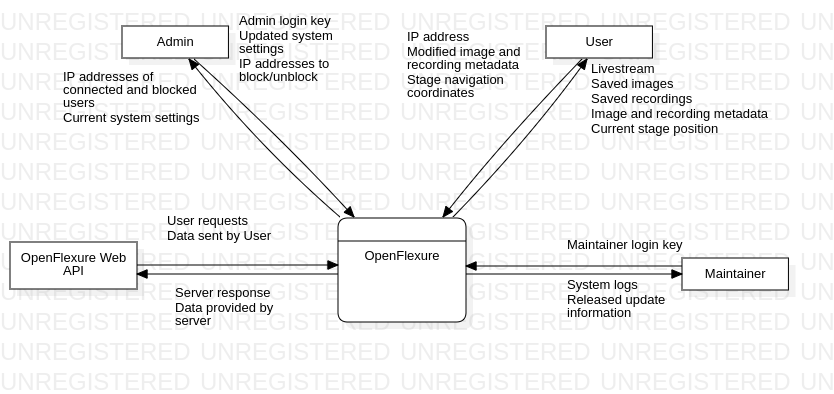
\includegraphics[scale=0.5]{Uml_Images/system_context_diagram}
	\caption{System Context Diagram for OpenFlexure}
	\label{fig:system_context_diagram}
\end{figure}


\subsubsection{Use-Case Diagram}
\begin{figure}[H]
	\centering
	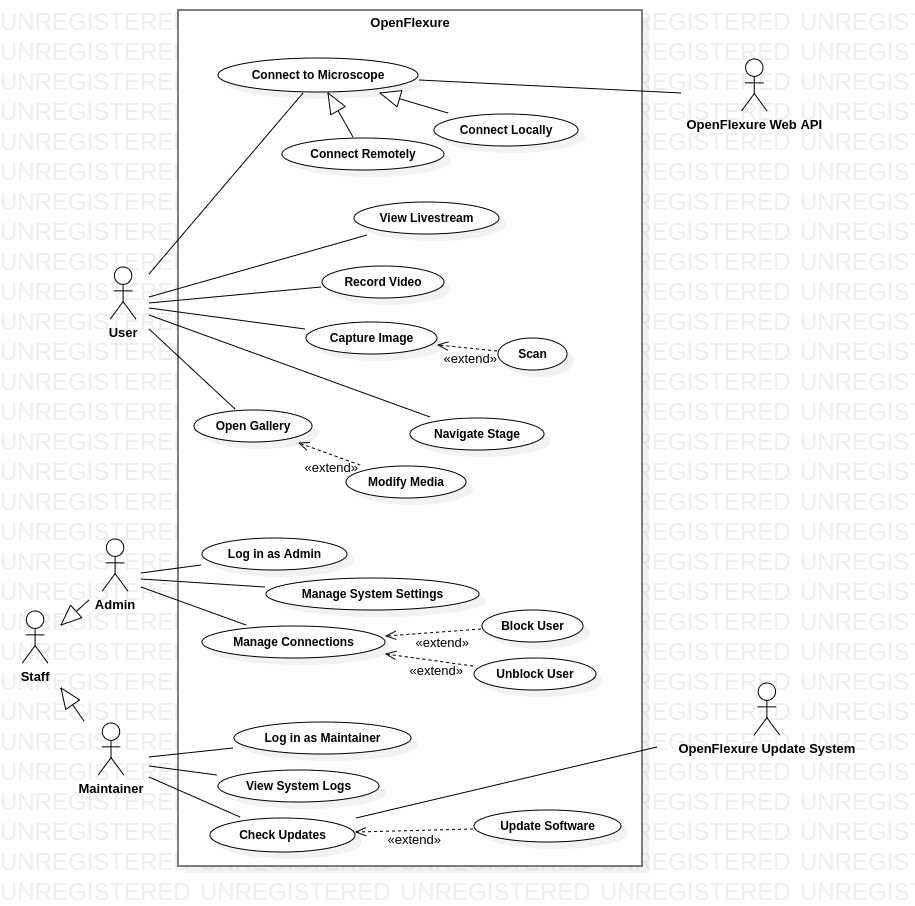
\includegraphics[scale=0.5]{Uml_Images/use_case_diagram}
	\caption{Use Case Diagram for OpenFlexure}
	\label{fig:use_case_diagram}
\end{figure}


\subsubsection{Use-Case Descriptions}
\begin{table}[H]
     \centering
     \begin{tabular}{|l|C|}
         \hline
          \textbf{Use-Case Name} & Connect to Microscope \\
         \hline
          \textbf{Actors} & User \\ 
         \hline
          \textbf{Description} & The user connects to the microscope's server. \\ 
         \hline
          \textbf{Data} & IP address of the user's computer\\ 
         \hline
          \textbf{Preconditions} & 
          Desktop application must be running. \\
         \hline
          \textbf{Stimulus} & The user clicks on "Connect to server" button placed in the home screen of the desktop application.\\ 
         \hline
          \textbf{Basic Flow} & 
          Step 1 -- The popup window contains the connection screen is opened. \newline
          Step 2 -- The user chooses "Connect remotely" option from the option boxes. \newline
          Step 3 -- Desktop application searches for the nearby microscope servers and lists the found ones. \newline
          Step 4 -- The user selects one of the microscopes listed in. \newline
          Step 5 -- The user clicks on "Connect" button. \\
         \hline
          \textbf{Alternative Flow\#1} & 
          Step 2 -- The user chooses "Connect locally" option. \newline
          Step 3 -- The desktop application searches for the web api internally stored in the Raspberry Pi, and when it finds, "Connect" button becomes available. \newline
          Step 4 -- The user clicks on "Connect" button. \\
         \hline
          \textbf{Alternative Flow\#2} & - \\
         \hline
          \textbf{Exception Flow} & If desktop application cannot found any nearby servers or the web api, the system displays an error message saying that "No device were found". If the IP address of the user is blocked, the system displays an error message saying that "Your IP address is blocked".\\
         \hline
          \textbf{Post Conditions} & The user connects to the microscope. \\ 
         \hline
     \end{tabular}
     \caption{Connect to Microscope}
     \label{tab:connect_to_microscope}
 \end{table}
\begin{table}[H]
     \centering
     \begin{tabular}{|l|C|}
         \hline
          \textbf{Use-Case Name} & View Livestream \\
         \hline
          \textbf{Actors} & User \\ 
         \hline
          \textbf{Description} & The user views the live camera feed. \\ 
         \hline
          \textbf{Data} & Camera feed\\ 
         \hline
          \textbf{Preconditions} & 
          User must be connected to the system. \newline
          Camera connection must be provided. \\
         \hline
          \textbf{Stimulus} & The user clicks on "View" button. \\ 
         \hline
          \textbf{Basic Flow} & 
          Step 1 -- The user clicks on "View" button from the side pine. \newline
		  Step 2 -- Server reaches Raspberry Pi camera. \newline
		  Step 3 -- Camera livestream is displayed in graphical user interface. \\
         \hline
          \textbf{Alternative Flow\#1} & - \\
         \hline
          \textbf{Alternative Flow\#2} & - \\
         \hline
          \textbf{Exception Flow} & If the camera connection is not established, the system displays an error message saying that "Check the camera connection".\\
         \hline
          \textbf{Post Conditions} & The livestream is displayed. \\ 
         \hline
     \end{tabular}
     \caption{View Livestream}
     \label{tab:view_livestream}
 \end{table}
\begin{table}[H]
     \centering
     \begin{tabular}{|l|C|}
         \hline
          \textbf{Use-Case Name} & Record Video \\
         \hline
          \textbf{Actors} & User, OpenFlexure Microscope \\ 
         \hline
          \textbf{Description} & The user starts recording the livestream. \\ 
         \hline
          \textbf{Data} & Recorded video\\ 
         \hline
          \textbf{Preconditions} & 
		  The user must be connected to the system. \newline
		  Camera connection must be provided. \\
         \hline
          \textbf{Stimulus} & The user clicks on "Record" button.\\ 
         \hline
          \textbf{Basic Flow} & 
          Step 1 -- The user clicks on "Record" button from the side pane. \newline
          Step 2 -- The tab that contains live camera feed and menu for recording settings opens. \newline
          Step 3 -- When user wants to start recording the livestream, he/she clicks on "Start Recording" button placed in the menu. \newline
          Step 4 -- The system sends "record" command to the "Camera System". \newline
          Step 5 -- The system displays a blinking led to indicate the recording. \newline
          Step 6 -- The user clicks on "Stop Recording" button to stop the recording. \newline
          Step 7 -- The system receives the recording from the "Camera System" and displays it in a popup window. \newline
          Step 8 -- The user gives a name to the recording by filling the textbox placed in the popup window and specifies the time interval if he/she wants to cut the recording before saving it. \newline
		  Step 9 -- The user clicks on "Save" button to save the recording. \newline
		  Step 10 -- The system saves the video to the location specified in system settings and create database record for the video using the Database Management Interface. \\
         \hline
          \textbf{Alternative Flow\#1} & 
          Step 8 -- The user clicks on the "Exit" button placed in the popup window to exit without saving the recording. \\
         \hline
          \textbf{Alternative Flow\#2} & - \\
         \hline
          \textbf{Exception Flow} & If the user tries to save the recording without naming it, the system displays an error message. If there is not enough available storage to store the recording, the system displays an error message.\\
         \hline
          \textbf{Post Conditions} & The recording is saved to the location specified in the settings and the popup window is closed. \\ 
         \hline
     \end{tabular}
     \caption{Record Video}
     \label{tab:record_video}
 \end{table}
\begin{table}[H]
     \centering
     \begin{tabular}{|l|C|}
         \hline
          \textbf{Use-Case Name} & Capture Image \\
         \hline
          \textbf{Actors} & User, OpenFlexure Microscope \\ 
         \hline
          \textbf{Description} & The user captures the image on the screen. \\ 
         \hline
          \textbf{Data} & Captured image\\ 
         \hline
          \textbf{Preconditions} & 
          The user must be connected to the system. \newline
          Camera connection must be provided. \\
         \hline
          \textbf{Stimulus} & The user clicks on "Capture" button.\\ 
         \hline
          \textbf{Basic Flow} & 
          Step 1 -- The user clicks on "Capture" button from the side pane. \newline
          Step 2 -- The tab that contains live camera feed and menu for image settings opens. \newline
          Step 3 -- When user wants to capture the image on the screen, he/she clicks on "Capture image" button placed in the menu. \newline
          Step 4 -- The system sends "capture" command to the "Camera System". \newline
          Step 5 -- The system receives the captured image from the "Camera System" and displays it in a popup window. \newline
          Step 6 -- The user gives a name to the captured image by filling the textbox placed in the popup window. \newline
		  Step 7 -- The user clicks on "Save" button to save the captured image. \newline
		  Step 8 -- The system saves the image to the location specified in system settings and create database record for the image using the Database Management Interface. \\
         \hline
          \textbf{Alternative Flow\#1} & 
          Step 6 -- The user clicks on the "Exit" button to exit without saving the captured image. \\
         \hline
          \textbf{Alternative Flow\#2} & - \\
         \hline
          \textbf{Exception Flow} & If the user tries to save the image without naming it, the system displays an error message. If there is not available storage to store the image, the system displays an error message.\\
         \hline
          \textbf{Post Conditions} & The image is saved to the location specified in the system settings and the popup window is closed. \\ 
         \hline
     \end{tabular}
     \caption{Capture Image}
     \label{tab:capture_image}
 \end{table}
\begin{table}[H]
	\centering
	\begin{tabular}{|l|C|}
		\hline
		\textbf{Use-Case Name} & Scan \\
		\hline
		\textbf{Actors} & User, OpenFlexure Microscope \\ 
		\hline
		\textbf{Description} & The system generates a scan of the area bounded by the coordinates provided by the user.\\ 
		\hline
		\textbf{Data} & Generated scan\\ 
		\hline
		\textbf{Preconditions} & 
		The user must be connected to the system. \newline
		Camera connection must be provided. \newline
		Capture tab must be opened. \\ 
		\hline
		\textbf{Stimulus} & The user clicks on "Scan" button.\\ 
		\hline
		\textbf{Basic Flow} & 
		Step 1 -- The user opens "Capture" tab from the side pane. \newline
		Step 2 -- The user activates "Scan" option by clicking the option box placed in image settings menu. \newline
		Step 3 -- The textboxes showing the coordinates that define the boundary of the area to be scanned becomes available. \newline
		Step 4 -- The user types the coordinates to the textboxes. \newline
		Step 5 -- Until the entire area has been scanned, at each step, the system sends a command to the "Motor Control System" to move by the step size specified in system settings and to the "Camera System" to capture the current image. \newline
		Step 6 -- The system merges all captured images to generate a bigger image of the area and displays it in a popup window. \newline
        Step 7 -- The user gives a name to the generated scan. \newline
		Step 8 -- The user clicks on "Save" button to save the generated scan. \newline
		Step 9 -- The system saves the scan image to the location specified in system settings and create database record for the image using the Database Management Interface. \\
		\hline
		\textbf{Alternative Flow\#1} & 
		Step 7 -- The user clicks on the "Exit" button to exit without saving the scan. \\
		\hline
		\textbf{Alternative Flow\#2} & - \\
		\hline
		\textbf{Exception Flow} & If the user tries to save the scan without naming it, the system displays an error message. If there is no available storage, the system displays an error message.\\
		\hline
		\textbf{Post Conditions} & The scan is saved to the location specified in the system settings. \\ 
		\hline
	\end{tabular}
	\caption{Scan}
	\label{tab:scan}
\end{table}
\begin{table}[H]
     \centering
     \begin{tabular}{|l|C|}
         \hline
          \textbf{Use-Case Name} & Navigate Stage \\
         \hline
          \textbf{Actors} & User, OpenFlexure Microscope \\ 
         \hline
          \textbf{Description} & The user adjusts the position of the stage. \\ 
         \hline
          \textbf{Data} & Coordinates of the stage in x, y and z axes\\ 
         \hline
          \textbf{Preconditions} & 
          User must be connected to the system. \\
         \hline
          \textbf{Stimulus} & The user clicks on "Navigate" button.\\ 
         \hline
          \textbf{Basic Flow} & 
          Step 1 -- The user clicks on "Navigate" button from the side pane. \newline
          Step 2 -- Tab that contains live camera feed and navigation menu opens. \newline
          Step 3 -- The user chooses the new x, y and z coordinates by filling the three textboxes placed in navigation menu. \newline
		  Step 4 -- The user clicks on "Apply" button. \newline
		  Step 5 -- The system sends the given coordinates to the "Motor Controller" \\
         \hline
          \textbf{Alternative Flow\#1} & - \\
         \hline
          \textbf{Alternative Flow\#2} & - \\
         \hline
          \textbf{Exception Flow} & If the motor connection is not established, the system displays an error message saying that "Check the motor connection".\\
         \hline
          \textbf{Post Conditions} & The position of the stage is physically changed. \\ 
         \hline
     \end{tabular}
     \caption{Navigate Stage}
     \label{tab:navigate_stage}
 \end{table}
\begin{table}[H]
     \centering
     \begin{tabular}{|l|C|}
         \hline
          \textbf{Use-Case Name} & Open Gallery \\
         \hline
          \textbf{Actors} & User \\ 
         \hline
          \textbf{Description} & The user displays the saved images and recorded videos. \\ 
         \hline
          \textbf{Data} & Images, recordings and metadata\\ 
         \hline
          \textbf{Preconditions} & 
          User must be connected to the system. \\
         \hline
          \textbf{Stimulus} & The user clicks on "Gallery" button \\ 
         \hline
          \textbf{Basic Flow} & 
          Step 1 -- The user clicks on "Gallery" button from the side pane. \newline
          Step 2 -- The server reaches to the database and retrieves the media records with the user's IP address in the authorIPAddress field.
          \newline
          Step 3 -- The system displays a list of images and recordings in a new tab as a grid style gallery where each entry has thumbnail and metadata of the corresponding media. \\
         \hline
          \textbf{Alternative Flow\#1} &  - \\ 
         \hline
          \textbf{Alternative Flow\#2} & -\\
         \hline
          \textbf{Exception Flow} & If there is no saved media associated with the user, the system displays a message saying that "No saved media were found."\\
         \hline
          \textbf{Post Conditions} & The user views the media saved by him/her. \\ 
         \hline
     \end{tabular}
     \caption{Open Gallery}
     \label{tab:open_gallery}
 \end{table}
\begin{table}[H]
     \centering
     \begin{tabular}{|l|C|}
         \hline
          \textbf{Use-Case Name} & Modify Media \\
         \hline
          \textbf{Actors} & User \\ 
         \hline
          \textbf{Description} & The user modifies the saved media. \\ 
         \hline
          \textbf{Data} & Metadata of the saved images and recordings\\ 
         \hline
          \textbf{Preconditions} & 
          User must be connected to the system. \newline
          Gallery tab must be active \\
         \hline
          \textbf{Stimulus} & The user clicks on one of the media entries in the gallery. \\ 
         \hline
          \textbf{Basic Flow} & 
          Step 1 --  The user clicks the media entry he/she wants to modify in the gallery. \newline
          Step 2 -- The popup window contains metadata information of the clicked media opens. \newline
          Step 3 -- The user changes the metadata of the media. \newline
          Step 4 -- The user clicks on "Save" button to save the updated metadata. \newline
          Step 5 -- The system updates the corresponding database records using the Database Management Interface. \\
         \hline
          \textbf{Alternative Flow\#1} &            
          Step 3 -- The user clicks on "Delete" button. \newline
          Step 4 -- The media is deleted from the storage location and corresponding database records is deleted from the database. \\
         \hline
          \textbf{Alternative Flow\#2} & -\\
         \hline
          \textbf{Exception Flow} & - \\
         \hline
          \textbf{Post Conditions} & The media is either deleted or its metadata is updated. \\ 
         \hline
     \end{tabular}
     \caption{Modify Media}
     \label{tab:modify_media}
 \end{table}
\begin{table}[H]
     \centering
     \begin{tabular}{|l|C|}
         \hline
          \textbf{Use-Case Name} & Log in as Admin \\
         \hline
          \textbf{Actors} & Admin \\ 
         \hline
          \textbf{Description} & The admin connects to server with his/her login key.\\ 
         \hline
          \textbf{Data} & Admin login key\\ 
         \hline
          \textbf{Preconditions} & - \\
         \hline
          \textbf{Stimulus} & The admin sends login request to server using the terminal.\\ 
         \hline
          \textbf{Basic Flow} & 
          Step 1 -- The server receives the login request. \newline
          Step 2 -- The server asks for the admin login key. \newline
          Step 3 -- Maintainer types his/her login key to the terminal. \newline
          Step 4 -- The system reaches to the local database and verifies the given login key.   \newline
          Step 5 -- The system signs in the admin. \\
         \hline
          \textbf{Alternative Flow\#1} & - \\
         \hline
          \textbf{Alternative Flow\#2} & - \\
         \hline
          \textbf{Exception Flow} & If the given key is invalid, the system displays an error message saying that "Given key is invalid". The system saves the report of the failed login attempt and the IP address of the user to the system logs. Then, the flow starts again from Step 2. \\
         \hline
          \textbf{Post Conditions} & The admin command line interface opens. \\ 
         \hline
     \end{tabular}
     \caption{Log in as Admin}
     \label{tab:log_in_as_admin}
 \end{table}
\begin{table}[H]
     \centering
     \begin{tabular}{|l|C|}
         \hline
          \textbf{Use-Case Name} & Manage System Settings \\
         \hline
          \textbf{Actors} & Admin \\ 
         \hline
          \textbf{Description} & The admin manages and updates the system settings. \\ 
         \hline
          \textbf{Data} & Current settings, updated setting\\ 
         \hline
          \textbf{Preconditions} & 
		  The admin must be logged in. \\
         \hline
          \textbf{Stimulus} & The admin gives "manage settings" command using the admin command line interface. \\ 
         \hline
          \textbf{Basic Flow} & 
          Step 1 -- The system reaches to the local database and retrieve the system settings record. \newline    
          Step 2 -- The system displays the current settings as a table where each row consists of the setting name and current value of the setting. \newline
          Step 3 -- The admin gives "set \{setting name\} \{new value\}" command to change the value of the specified setting. \newline
          Step 4 -- The system reaches to database and changes the value of the given settings field. \\
         \hline
          \textbf{Alternative Flow\#1} &  - \\
         \hline
          \textbf{Alternative Flow\#2} & -\\
         \hline
          \textbf{Exception Flow} & - \\
         \hline
          \textbf{Post Conditions} & The system settings are updated. \\ 
         \hline
     \end{tabular}
     \caption{Manage System Settings}
     \label{tab:manage_system_settings}
 \end{table}
\begin{table}[H]
     \centering
     \begin{tabular}{|l|C|}
         \hline
          \textbf{Use-Case Name} & Manage Connections \\
         \hline
          \textbf{Actors} & Admin \\ 
         \hline
          \textbf{Description} & The admin views the list of connected and blocked users. \\ 
         \hline
          \textbf{Data} & IP addresses, types (user, maintainer or admin) and the statuses (connected, blocked) of the users. \\
         \hline
          \textbf{Preconditions} & 
          The admin must be logged in. \\
         \hline
          \textbf{Stimulus} & The admin gives "manage connections" command using the admin command-line interface.\\ 
         \hline
          \textbf{Basic Flow} & 
          Step 1 -- The system reaches to the database and gathers records of the connected and blocked users. \newline
          Step 2 -- The system displays the list of IP addresses, connection times and the statuses (connected, blocked) of the users. \\
         \hline
          \textbf{Alternative Flow\#1} & -\\
         \hline
          \textbf{Alternative Flow\#2} & - \\
         \hline
          \textbf{Exception Flow} & If there is no connected or blocked user, the system displays an error message saying that "No data were found".\\
         \hline
          \textbf{Post Conditions} & The admin views the connected and blocked users. \\ 
         \hline
     \end{tabular}
     \caption{Manage Connections}
     \label{tab:manage_connections}
 \end{table}
\begin{table}[H]
     \centering
     \begin{tabular}{|l|C|}
         \hline
          \textbf{Use-Case Name} & Block User \\
         \hline
          \textbf{Actors} & Admin \\ 
         \hline
          \textbf{Description} & The admin blocks a user with given IP address. \\ 
         \hline
          \textbf{Data} & IP address of the user\\ 
         \hline
          \textbf{Preconditions} & 
          The admin must be logged in. \newline
          The admin must have given the "manage connections" command beforehand.\\
         \hline
          \textbf{Stimulus} & The admin types "block user" command in the admin command-line interface.\\ 
         \hline
          \textbf{Basic Flow} & 
          Step 1 -- The system asks for the IP address of the user to block. \newline
          Step 2 -- The admin gives the IP address of the user obtained from the list displayed after "manage connections" command. \newline
          Step 3 -- Server reaches to the database and sets the blockStatus field of the user record with the given IP Address as "blocked" \\
         \hline
          \textbf{Alternative Flow\#1} & -\\
         \hline
          \textbf{Alternative Flow\#2} & - \\
         \hline
          \textbf{Exception Flow} & If there is no connected user with the given IP address, the system displays an error message saying that "Invalid Ip address". If the user with the given IP address  has already been blocked, the system displays an error message saying that "The given IP address has already been blocked".\\
         \hline
          \textbf{Post Conditions} & The user with the given IP address will not be able to connect to the server until it is unblocked.\\ 
         \hline
     \end{tabular}
     \caption{Block User}
     \label{tab:block_user}
 \end{table}
\begin{table}[H]
     \centering
     \begin{tabular}{|l|C|}
         \hline
          \textbf{Use-Case Name} & Unblock User \\
         \hline
          \textbf{Actors} & Admin \\ 
         \hline
          \textbf{Description} & The admin unblocks a user with given IP address. \\ 
         \hline
          \textbf{Data} & IP address of the user\\ 
         \hline
          \textbf{Preconditions} & 
          The admin must be logged in. \newline
          The admin must have given the "manage connections" command beforehand.\\
         \hline
          \textbf{Stimulus} & The admin types "unblock user" command in the admin command-line interface.\\ 
         \hline
          \textbf{Basic Flow} & 
          Step 1 -- The system asks for the IP address of the user to unblock. \newline
          Step 2 -- The admin gives the IP address of the user obtained from the list displayed after "manage connections" command. \newline
          Step 3 -- Server reaches to the database and sets the blockStatus field of the user record with the given IP Address as "unblocked" \\
         \hline
          \textbf{Alternative Flow\#1} & -\\
         \hline
          \textbf{Alternative Flow\#2} & - \\
         \hline
          \textbf{Exception Flow} & If there is no blocked user with the given IP address, the system displays an error message saying that "No blocked users were found". \\
         \hline
          \textbf{Post Conditions} & The user with the given IP address will be able to connect to the server again. \\ 
         \hline
     \end{tabular}
     \caption{Unblock User}
     \label{tab:unblock_user}
 \end{table}
\begin{table}[H]
     \centering
     \begin{tabular}{|l|C|}
         \hline
          \textbf{Use-Case Name} & Log in as Maintainer \\
         \hline
          \textbf{Actors} & Maintainer \\ 
         \hline
          \textbf{Description} & The maintainer connects to server with his/her login key.\\ 
         \hline
          \textbf{Data} & Maintainer login key\\ 
         \hline
          \textbf{Preconditions} & - \\
         \hline
          \textbf{Stimulus} & The maintainer sends login request to server from the terminal.\\ 
         \hline
          \textbf{Basic Flow} & 
          Step 1 -- The server receives the login request. \newline
          Step 2 -- The server asks for the maintainer login key. \newline
          Step 3 -- Maintainer types his/her login key to the terminal. \newline
          Step 4 -- The system reaches to the local database and verifies the given login key.   \newline
          Step 5 -- The system signs in the maintainer. \\
         \hline
          \textbf{Alternative Flow\#1} & - \\
         \hline
          \textbf{Alternative Flow\#2} & - \\
         \hline
          \textbf{Exception Flow} & If the given key is invalid, the system displays an error message saying that "Given key is invalid". The system saves the log of the failed login attempt and the IP address of the user to the database. Then, the flow starts again from Step 2. \\
         \hline
          \textbf{Post Conditions} & The maintainer command-line interface opens. \\ 
         \hline
     \end{tabular}
     \caption{Log in as Maintainer}
     \label{tab:log_in_as_maintainer}
 \end{table}
\begin{table}[H]
     \centering
     \begin{tabular}{|l|C|}
         \hline
          \textbf{Use-Case Name} & View system logs \\
         \hline
          \textbf{Actors} & Maintainer \\ 
         \hline
          \textbf{Description} & The maintainer can list and view the system logs sorted by their dates.\\ 
         \hline
          \textbf{Data} & System logs\\ 
         \hline
          \textbf{Preconditions} & 
          Maintainer must be logged in. \\
         \hline
          \textbf{Stimulus} & The maintainer gives "view logs" command using the command-line interface.\\ 
         \hline
          \textbf{Basic Flow} & 
          Step 1 -- The server takes the request. \newline
          Step 2 -- The server gathers the system logs from the database. \newline
          Step 3 -- The system displays the system logs in command-line interface. \\
         \hline
          \textbf{Alternative Flow\#1} & - \\
         \hline
          \textbf{Alternative Flow\#2} & - \\
         \hline
          \textbf{Exception Flow} & If there is no system logs in database, the system displays a message saying that "No system logs were found". \\
         \hline
          \textbf{Post Conditions} & The system logs are displayed in the maintainer's interface. \\ 
         \hline
     \end{tabular}
     \caption{View System Logs}
     \label{tab:view_system_logs}
 \end{table}
\begin{table}[H]
     \centering
     \begin{tabular}{|l|C|}
         \hline
          \textbf{Use-Case Name} & Check Updates \\
         \hline
          \textbf{Actors} & Maintainer, OpenFlexure Update System \\ 
         \hline
          \textbf{Description} & The maintainer checks for the software updates.\\ 
         \hline
          \textbf{Data} & System's current software version, released update information\\
         \hline
          \textbf{Preconditions} & 
          Maintainer must be logged in. \\
         \hline
          \textbf{Stimulus} & The maintainer gives "check updates" command using the command line interface.\\ 
         \hline
          \textbf{Basic Flow} & 
          Step 1 -- The server retrieves the version number of the software from the database. \newline
          Step 2 -- The server sends the current version number of the software to the OpenFlexure Update System. \newline
          Step 3 -- The server receives the information about the latest update returned by the OpenFlexure Update System. \newline
          Step 4 -- The server displays the version number, size, release date and changelog of the update in command-line interface. \\
         \hline
          \textbf{Alternative Flow\#1} & - \\
         \hline
          \textbf{Alternative Flow\#2} & - \\
         \hline
          \textbf{Exception Flow} & If the system is already using the latest version, an error message saying that "No updates were found" is displayed. \\
         \hline
          \textbf{Post Conditions} & Information about the latest update is displayed in the command-line interface. \\ 
         \hline
     \end{tabular}
     \caption{Check Updates}
     \label{tab:check_updates}
 \end{table}
\begin{table}[H]
     \centering
     \begin{tabular}{|l|C|}
         \hline
          \textbf{Use-Case Name} & Update Software \\
         \hline
          \textbf{Actors} & Maintainer, OpenFlexure Update System \\ 
         \hline
          \textbf{Description} & The maintainer updates the system software.\\ 
         \hline
          \textbf{Data} & Installable update package\\ 
         \hline
          \textbf{Preconditions} & 
          Maintainer must be logged in. \newline
          Maintainer must have given the "check updates" command beforehand.\\
         \hline
          \textbf{Stimulus} & The maintainer gives "update" command using the command line interface.\\ 
         \hline
          \textbf{Basic Flow} & 
          Step 1 -- The server requests the update package from the OpenFlexure Update System. \newline
          Step 2 -- The package is downloaded to the Raspberry Pi. \newline
          Step 3 -- The server installs the downloaded package. \newline
          Step 4 -- The server saves the version number and the release date of the update to the corresponding database table. \\
         \hline
          \textbf{Alternative Flow\#1} & - \\
         \hline
          \textbf{Alternative Flow\#2} & - \\
         \hline
          \textbf{Exception Flow} & If an error is encountered during the installation, for example, if the downloaded package is corrupted, the system saves the detailed error log into the database. \\
         \hline
          \textbf{Post Conditions} & The system is updated to the latest version. \\ 
         \hline
     \end{tabular}
     \caption{Update Software}
     \label{tab:update_software}
 \end{table}

\subsection{Composition View}
The Composition View section provides information about the components of the system. Detailed information can be found corresponding parts of the section.
\subsubsection{Component Diagram}
\begin{figure}[H]
	\centering
	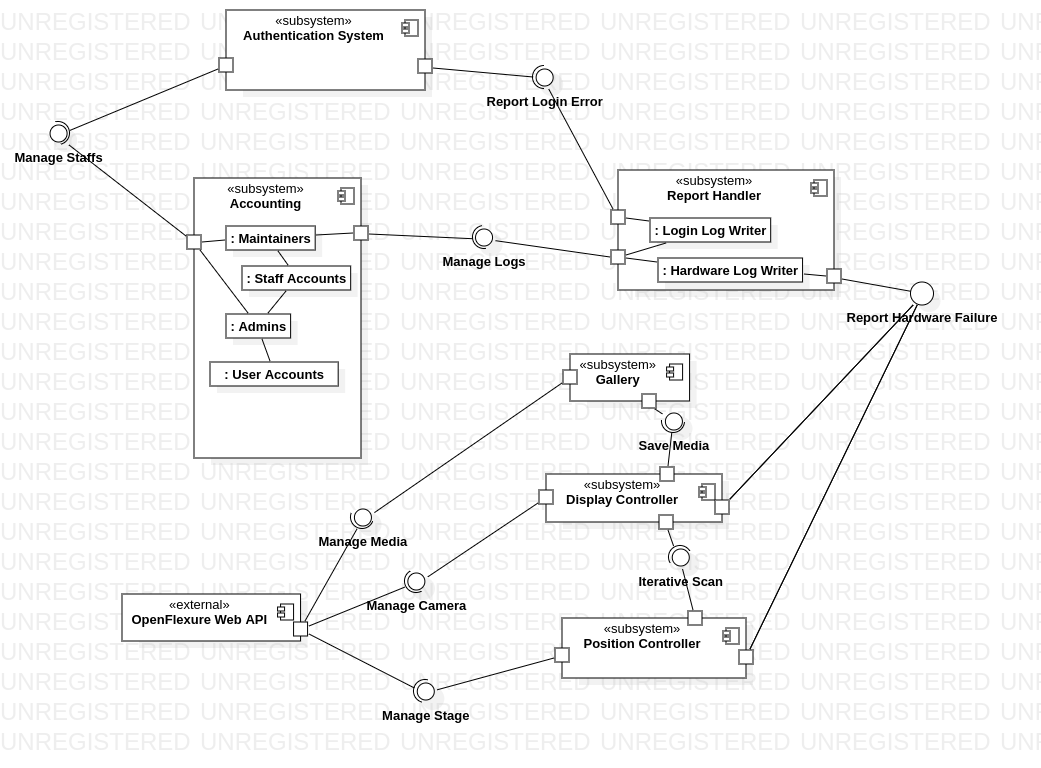
\includegraphics[scale=0.4]{Uml_Images/component_diagram}
	\caption{Component Diagram for OpenFlexure}
	\label{fig:component_diagram}
\end{figure}

\subsubsection{Deployment Diagram}
\begin{figure}[H]
	\centering
	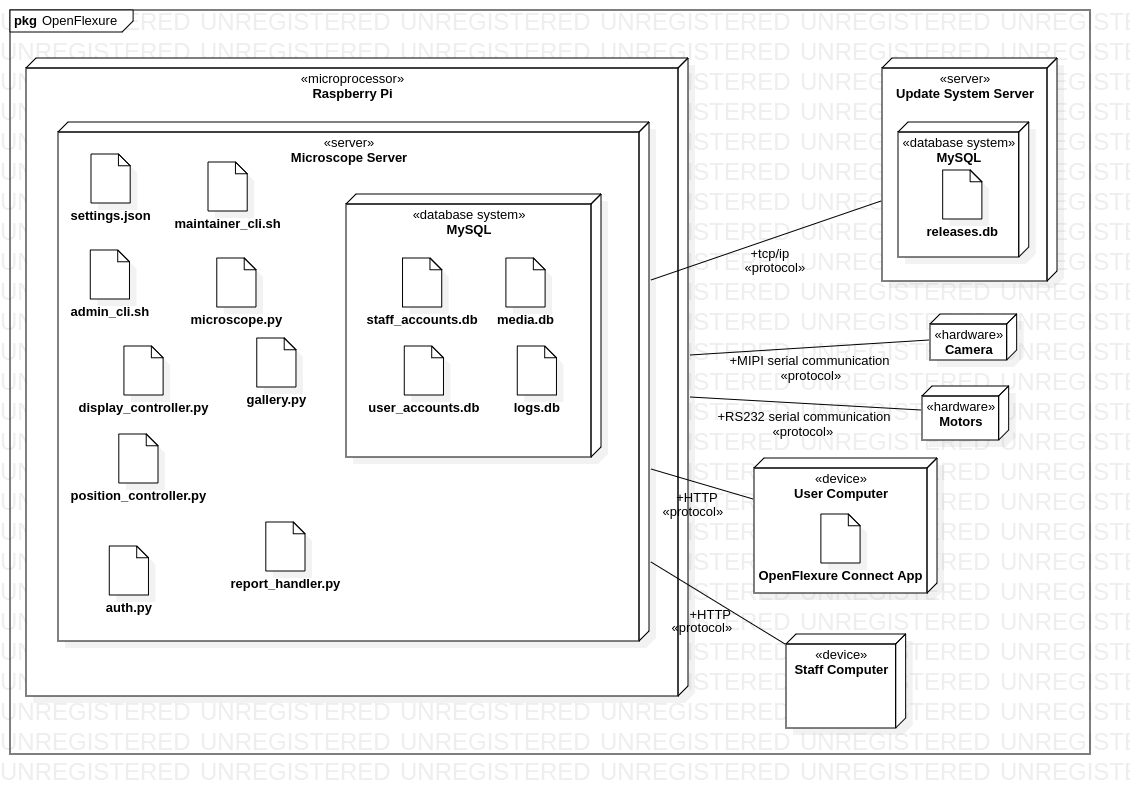
\includegraphics[scale=0.4]{Uml_Images/deployment_diagram}
	\caption{Deployment Diagram for OpenFlexure}
	\label{fig:deployment_diagram}
\end{figure}

\subsubsection{Design Rationale}
\paragraph{Component Diagram}
\begin{itemize}
	\item To allow the admins to use Block User and Unblock User functions defined in use-case diagram, Admins part is associated with the User Accounts part.
	\item To allow the admins to use Block User and Unblock User functions defined in use-case diagram, Admins part is associated with the User Accounts part.
	\item To allow the Authentication Systems to check the provided password information, Accounting provides an interface.
	\item Report Handler provides two different interfaces which are used by the Authentication System, Position Controller and Display Controller to write and store Login related and Hardware related issues.
	\item To be able to store the media (images and videos) generated by the Display Controller, Gallery provides an interface.
\end{itemize}
\paragraph{Deployment Diagram}
\begin{itemize}
	\item MySQL is used as database management system to store System Logs, Staff Accounts, User Connection Records and saved Media Metadata.
	\item System Settings are stored in json file, since it is easier and faster to process json file.
	\item To provide Admin Commmand-line Interface and Maintainer Command-line Interface two bash programs are stored in the server, admin\_cli.sh and maintainer\_cli.sh, respectively.
	\item Authentications of the staff personal are done by auth.py
	\item For Raspberry PI Camera hardware and Motor hardware MIPI and RS232 serial communication protocols are used.
\end{itemize}

\subsection{Information View}
The Information View section contains information about the organization and the relations of the data stored in the system.
\subsubsection{Class Diagram}

\begin{figure}[H]
	\centering
	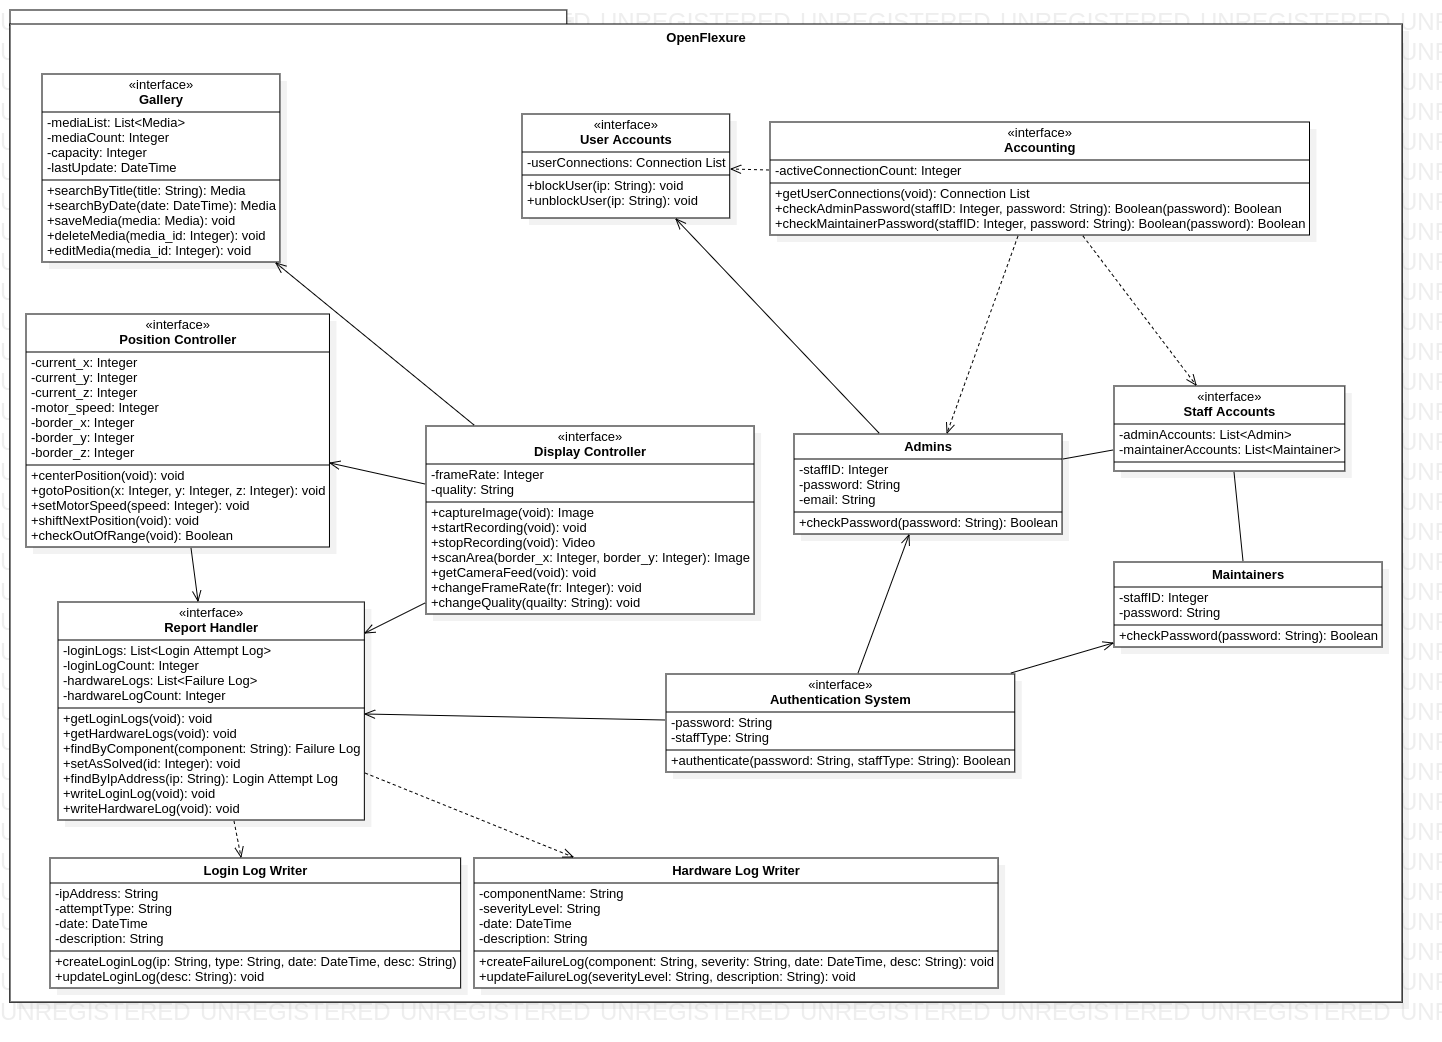
\includegraphics[scale=0.3]{Uml_Images/interface_class_diagram}
	\caption{Interface Class Diagram for OpenFlexure}
	\label{fig:interface_class_diagram}
\end{figure}

\begin{table}[H]
	\centering
	\begin{tabular}{|l|C|}
		\hline
		\textbf{Operation}   &  \textbf{Description}\\
		\hline
		searchByTitle   &  returns the media with given title\\
		\hline
		searchByDate   &  returns the media with given date\\
		\hline
		saveMedia  &  saves the given media to the gallery media list\\
		\hline
		deleteMedia   &  delete the media with given id from the gallery media list\\
		\hline
		editMedia   &  edits the media with given id\\
		\hline
		centerPosition   &  positions the stage to the center\\
		\hline
		gotoPosition   &  positions the stage to the point with the given coordinates\\
		\hline
		setMotorSpeed  &  sets the motor speed\\
		\hline
		shiftNextPosition  &  shifts the stage position to the next one by incrementing the current coordinates\\
		\hline
		checkOutOfRange  &  checks if the current coordinates are out of range\\
		\hline
		captureImage  &  captures the displayed livestream and returns the captured image\\
		\hline
		startRecording   &  starts recording the livestream\\
		\hline
		stopRecording   &  stops the ongoing recording and returns the recorded video\\
		\hline
		scanArea & scans the area with the given border coordinates and returns it as image\\
		\hline
		getCameraFeed & streams the live camera feed \\
		\hline
		changeFrameRate & changes the frame rate of the camera\\
		\hline
		changeQuality & changes the quality of the camera\\
		\hline
		getLoginLogs & returns the list of Login Attempt Logs\\
		\hline
		getHardwareLogs & returns the list of Failure Logs\\
\hline
		findByComponent & returns the Failure Log with the given component name\\
\hline
		setAsSolved & sets the status of the log with given id as solved\\
\hline
		findByIpAddress & returns the Login Attempt Log with the given component name\\
\hline
		writeLoginLog & writes the login log created by Login Log Writer to the loginLogs list\\
\hline
		writeHardwareLog & writes the hardware log created by Hardware Log Writer to the hardwareLogs list\\
\hline
		createLoginLog & creates a Login Attempt Log and fills it with the given parameters\\
\hline
	\end{tabular}
\end{table}

\begin{table}[H]
	\centering
	\begin{tabular}{|l|C|}
		\hline
	updateLoginLog & updates the Login Attempt Log with the given id\\
	\hline
	createFailureLog & creates a Failure Log and fills it with the given parameters\\
	\hline
	updateFailureLog & updates the Failure Log with the given id\\
	\hline
	authenticate & checks the password of the user with given staff type and authenticates him/her\\
	\hline
	getUserConnections & returns the list of Connections \\
	\hline
	checkAdminPassword & compares the given password with the password of the admin with given staffID and returns the result of the comparison \\
	\hline
	checkMaintainerPassword & compares the given password with the password of the maintainer with given staffID and returns the result of the comparison \\
	\hline
	blockUser & sets the blockStatus of the user with the given ip as True \\
	\hline
	unblockUser & sets the blockStatus of the user with the given ip as False \\
	\hline
	checkPassword & compares the given password with the password of the admin/maintainer \\
	\hline
	\end{tabular}
	\caption{Operation Descriptions}
	\label{tab:operation_descriptions}
\end{table}

\begin{figure}[H]
	\centering
	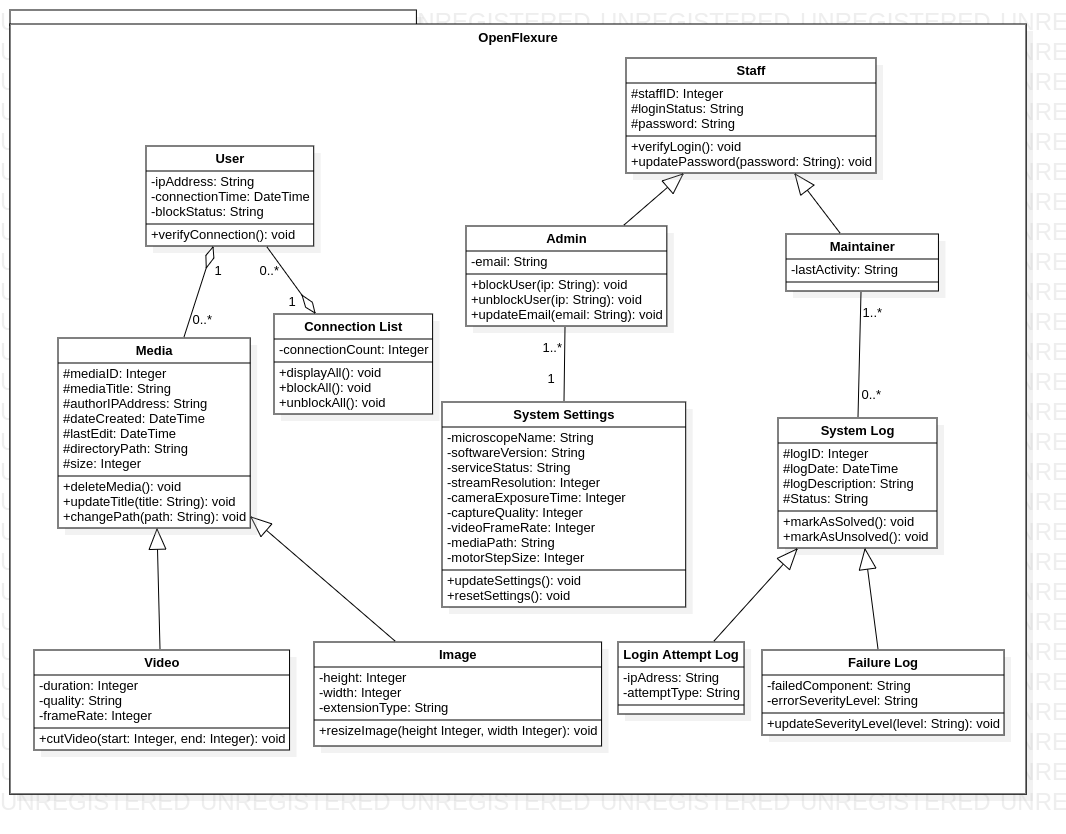
\includegraphics[scale=0.4]{Uml_Images/db_class_diagram}
	\caption{Database Class Diagram for OpenFlexure}
	\label{fig:db_class_diagram}
\end{figure}

\subsubsection{Database Operations}
\begin{table}[H]
	\centering
	\begin{tabular}{|p{5cm}|p{7cm}|}
		\hline
		\textbf{Operation} & \textbf{CRUD Operations} \\
		\hline
		verifyLogin &
		CREATE:\newline
		READ: \texttt{Staff} \newline
		UPDATE: \texttt{Staff} \newline
		DELETE: \\
		\hline
		updatePassword &
		CREATE:\newline
		READ: \newline
		UPDATE: \texttt{Staff}\newline
		DELETE: \\
		\hline
		updateEmail &
		CREATE:\newline
		READ: \newline
		UPDATE: \texttt{Admin}\newline
		DELETE: \\
		\hline
		blockUser &
		CREATE:\newline
		READ: \newline
		UPDATE: \texttt{User}\newline
		DELETE: \\
		\hline
		unblockUser &
		CREATE:\newline
		READ: \newline
		UPDATE: \texttt{User}\newline
		DELETE: \\
		\hline
		updateSettings &
		CREATE:\newline
		READ: \newline
		UPDATE: \texttt{Settings}\newline
		DELETE: \\
		\hline
		resetSettings &
		CREATE:\newline
		READ: \texttt{Settings}\newline
		UPDATE: \texttt{Settings}\newline
		DELETE: \\
		\hline
		markAsSolved &
		CREATE:\newline
		READ: \newline
		UPDATE: \texttt{System Log}\newline
		DELETE: \\
		\hline
	\end{tabular}
\end{table}

\begin{table}[H]
	\centering
	\begin{tabular}{|p{5cm}|p{7cm}|}
		\hline
		markAsUnsolved &
		CREATE:\newline
		READ: \newline
		UPDATE: \texttt{System Log}\newline
		DELETE: \\
		\hline
		updateSeverityLevel &
		CREATE:\newline
		READ: \newline
		UPDATE: \texttt{Failure Log}\newline
		DELETE: \\
		\hline
		verifyConnection &
		CREATE: \newline
		READ: \texttt{User}\newline
		UPDATE: \texttt{User}\newline
		DELETE: \\
		\hline
		deleteMedia &
		CREATE: \newline
		READ:  \newline
		UPDATE: \newline
		DELETE: \texttt{Media} \\
		\hline
		updateTitle &
		CREATE: \newline
		READ:  \newline
		UPDATE: \texttt{Media} \newline
		DELETE:  \\
		\hline
		changePath &
		CREATE: \newline
		READ:  \newline
		UPDATE: \texttt{Media} \newline
		DELETE:  \\
		\hline
		cutVideo &
		CREATE: \newline
		READ:  \newline
		UPDATE: \texttt{Video} \newline
		DELETE:  \\
		\hline
		resizeImage &
		CREATE: \newline
		READ:  \newline
		UPDATE: \texttt{Image} \newline
		DELETE:  \\
		\hline
		displayAll &
		CREATE: \newline
		READ: \texttt{Connection List}, \texttt{User}\newline
		UPDATE: \newline
		DELETE: \\
		\hline
	\end{tabular}
\end{table}
\begin{table}[H]
	\centering
	\begin{tabular}{|p{5cm}|p{7cm}|}
		\hline
		blockAll &
		CREATE: \newline
		READ: \texttt{Connection List} \newline
		UPDATE: \texttt{User} \newline
		DELETE: \\
		\hline
		unblockAll &
		CREATE: \newline
		READ: \texttt{Connection List} \newline
		UPDATE: \texttt{User} \newline
		DELETE: \\
		\hline
	\end{tabular}
	\caption{CRUD Operations}
	\label{tab:crud_operations}
\end{table}

\subsubsection{Design Rationale}
\paragraph{Interface Class Diagram}
\begin{itemize}
	\item Report Handler is responsible for creating and storing logs related to hardware failures and login errors.
	\item Both Display Controller and Position Controller associated with the Report Handler to report hardware related problems.
	\item Authentication System is associated with the Report Handler to report suspicious login attempts.
	\item To allow the maintainers to use View System Logs function defined in use-case diagram, Maintainers component uses the interface provided by the Report Handler.
	\item To allow the admins to use Block User and Unblock User functions defined in use-case diagram, Admins part is associated with the User Accounts part.
	\item To be able to store the captured images, scans and recorded videos, Display Controller is associated with the Gallery.
\end{itemize}
\paragraph{Database Class Diagram}
\begin{itemize}
	\item For easy and fast usability of the microscope, users do not have to authenticate to the system. Therefore, for user records, password information is omitted.
	\item To avoid repetition of the attributes, Media, System Log and Staff parent classes are defined. 
	\item To be able to handle different types of errors, Login Attempt Log and Failure Log classes are created.
	\item To allow the maintainer to use View System Logs function defined in use-case diagram, Maintainer and System Logs classes are linked to each other.
\end{itemize}

\subsection{Interface View}
The Interface View section provides information about the internal and external interfaces of the system.
\subsubsection{Internal Interfaces}
\paragraph{Interface between Accounting and Authentication System}
The interface provided by Accounting component is used by the Authentication System to verify the provided staffID and password.
\subparagraph{Design Rationale:}
\begin{itemize}
	\item Authentication System sends the given staffID and password parameters to the Accounting component.
	\item Based on the type of the staff Accounting checks the password using checkPassword operation belongs to either Admins or Maintainers parts.
	\item Returns the result of the checkPassword operation.
\end{itemize}
\paragraph{Interface between Authentication System and Report Handler}
The interface provided by the Report Handler is used by the Authentication System to report suspicious and wrong login attempts.
\subparagraph{Design Rationale:}
\begin{itemize}
	\item If the boolean result returned by the Accounting, Authentication System sends the provided information to the Report Handler.
	\item Report Handler saves the Login Attempt Log created by the Login Log Writer part in the loginLogs list. 
\end{itemize}
\paragraph{Interface between Accounting and Report Handler}
The interface provided by the Report Handler is used by the Accounting and especially its subcomponent Maintainers to display and check the written System Logs.
\subparagraph{Design Rationale:}
\begin{itemize}
	\item Report Handler provides the loginLogs list and hardwareLogs list to the Accounting and specifically Maintainers part to allow maintainers to use View System Logs function.
\end{itemize}
\paragraph{Interface between Report Handler and Display Controller and Position Controller}
The interface provided by the Report Handler is used by both Display and Position Controllers to report any hardware related technical issues.
\subparagraph{Design Rationale:}
\begin{itemize}
	\item Since Display and Position Controllers are related to hardware devices (camera and motors), it is possible to have hardware related issues. This interface is for handling the hardware related problems.
	\item Report Handler saves the Failure Log created by the Hardware Log Writer part in the hardwareLogs list. 
\end{itemize}
\paragraph{Interface between Display Controller and Position Controller}
The interface provided by the Position Controller is used by the Display Controller for the scanArea operation. In this operation by using this interface Display Controller is able to iteratively move the camera position to scan the area.
\subparagraph{Design Rationale:}
\begin{itemize}
	\item To be able to use Scan function defined in the use-case diagram Display Controller serves scanArea function.
	\item To use the scanArea function position of the stage should be shifted iteratively. Position Controller serves this interface to allow Display Controller to shift stage position in each iteration.
\end{itemize}
\paragraph{Interface between Display Controller and Gallery}
The interface provided by the Gallery is used by the Display Controller to save the captured Images, scans, recorded videos.
\subparagraph{Design Rationale:}
\begin{itemize}
	\item Display Controller is responsible to implement Capture Image, Record Video and Scan functions defined in use-case diagram.
	\item To be able to store the media generated by the Display Controller, Gallery serves this interface.
\end{itemize}
\subsubsection{External Interfaces}
	\paragraph{User Interfaces}
	\begin{itemize}
		\item \textbf{User Web Interface} \\
		Users use a web interface written in javascript using Vue.js framework which is running inside the local microscope server. User can reach to  the User Web Interface by just typing the ip address and designated port of the microscope's server in their browser. Users are able to control the microscope and view the camera feed using the user interface. User Web Interface provides live stream camera feed, navigation menu to change the position of the stage and gallery to view and update the saved media. \\
		\textbf{Design Rationale:} 
		\begin{enumerate}
			\item User web interface has a very simple design to allow inexperienced users to use the provided features easily.
			\item It has a help window that contains solutions for the frequently faced problems to guide users faced with such problems.
			\item The icons have been placed inside the tab buttons in addition to button labels to ensure that the desired feature can be found easily.
		\end{enumerate}
		\begin{figure}[H]
			\centering
			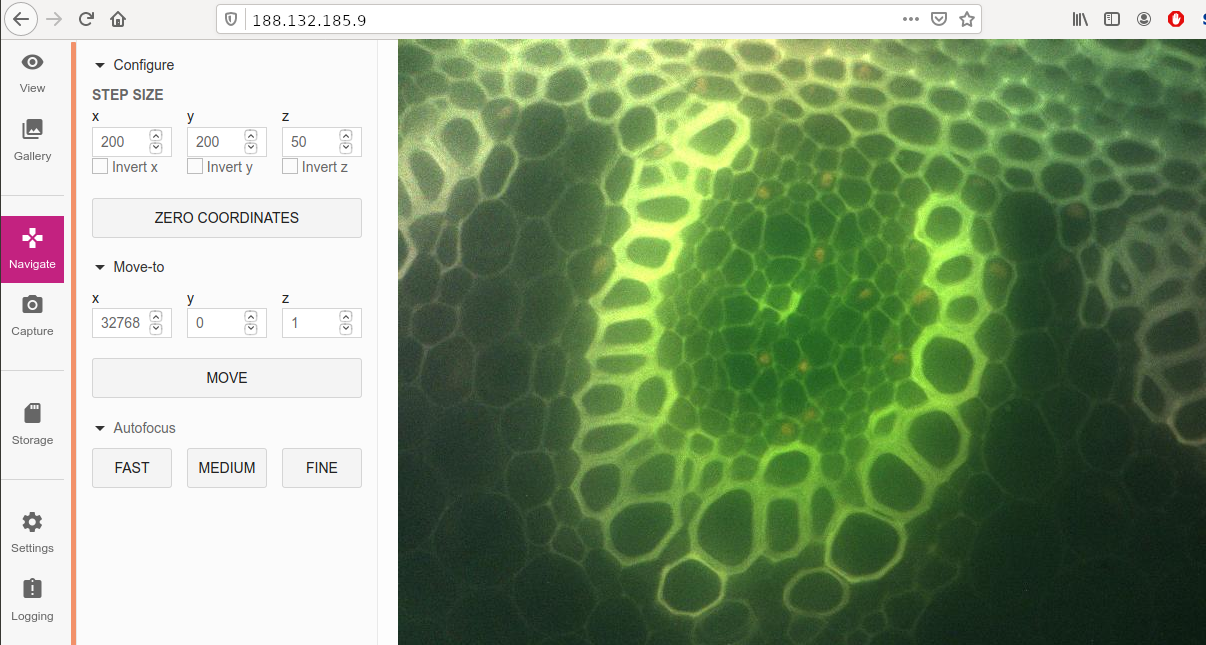
\includegraphics[scale=0.3]{Figures/user_web_interface}
			\caption{OpenFlexure User Web Interface}
			\label{fig:user_web_interface}
		\end{figure}
		\item \textbf{Admin Command-line Interface} \\
		System administrators use a command-line interface to manage the system. Administrators are able to list the detailed information about connected/blocked users such as User IPs, block/unblock status, and connection time. Using the commands provided by this interface, the administrators can view/manage/update system settings and block/unblock users. Admin command-line interface is provided by a bash script placed inside the local microscope server and starts to run when an admin connects to the microscope using SSH. \\
		\textbf{Design Rationale:} 
		\begin{enumerate}
			\item The reason to use a command-line interface rather than GUI is related to speed. Administrators should be able to apply their actions immediately. Since the command-line interface is a more quick way to apply actions, it is preferred over GUI.
		\end{enumerate}
		\begin{figure}[H]
			\centering
			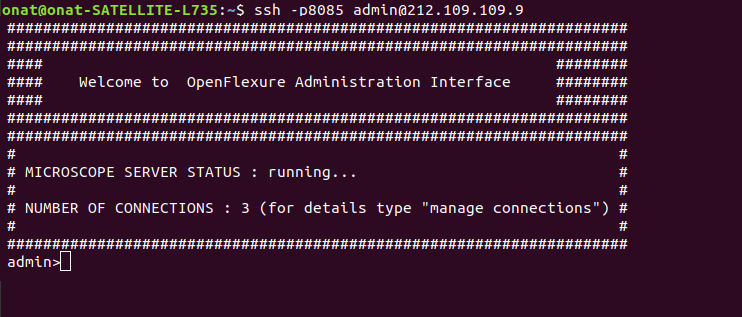
\includegraphics[scale=0.5]{Figures/admin_interface}
			\caption{OpenFlexure Administration Command-line Interface}
			\label{fig:system_admin_management_interface}
		\end{figure}
		\item \textbf{Maintainer Command-line Interface} \\
		Similar to system administrators, maintainers use a separate maintainer command-line interface to do their tasks, due to the similar reasons. Since the permissions of the maintainers are limited to viewing released updates, updating the system and retrieving the system logs, commands available to maintainers are also limited. Maintainers can list saved error logs, system details such as the current software version and the information about the latest software updates. Furthermore, maintainers are also able to update the system software using the command provided by this interface. Maintainer command-line interface is provided by a bash script placed inside the local microscope server and starts to run when a maintainer connects to the microscope using SSH.
	\end{itemize}
	\textbf{Design Rationale:} 
	\begin{enumerate}
		\item The reason to use a command-line interface rather than GUI is related to speed. Maintainers should be able to apply their actions immediately. Since the command-line interface is a more quick way to apply actions, it is preferred over GUI.
	\end{enumerate}
	\paragraph{System/Service Interfaces}
	\paragraph{Interface between Web API and Gallery}
	The interface provided by the Gallery is used by the Web API when a user sends a request to the Web API to display/edit/manage the saved media materials.
	\subparagraph{Design Rationale:}
	\begin{itemize}
		\item User sends a request to the Web API to view/edit the stored media.
		\item To allow the Web API to use the media facilities that user wants to use, Gallery provides this interface and based on the request sent to the Web API, corresponding operation of the Gallery is activated.
		\item This interface is related to the Open Gallery and Modify Media functions defined in the use-case diagram.
	\end{itemize}
	\paragraph{Interface between Web API and Position Controller}
	The interface provided by the Position Controller is used by the Web API when a user sends a request to the Web API to move the position of the stage.
	\subparagraph{Design Rationale:}
	\begin{itemize}
		\item User sends a request to the Web API to navigate the positions of the microscope stage.
		\item To allow the Web API to change the position of the stage to the desired position, Position Controller provides this interface and changes the positions of the stage using the provided coordinates.
		\item This interface is related to the Navigate Stage function defined in the use-case diagram.
	\end{itemize}
	\paragraph{Interface provided Web API and Display Controller}
	The interface provided by the Display Controller is used by the Web API when a user sends a request to display the livestream, capture the current view, record to the livestream or scan an area.
	\subparagraph{Design Rationale:}
	\begin{itemize}
		\item User sends a request to the Web API to use facilities provided by the Display Controller such as viewing livestream, capturing images, recording videos etc.
		\item To allow the Web API to use the mentioned facilities that user wants to use, Display Controller provides this interface and based on the request sent to the Web API, corresponding operation of the Display Controller is activated.
		\item This interface is related to the View Livestream, Capture Image, Record Video and Scan functions defined in the use-case diagram.
	\end{itemize}

\subsubsection{Sequence Diagrams}
\begin{figure}[H]
	\centering
	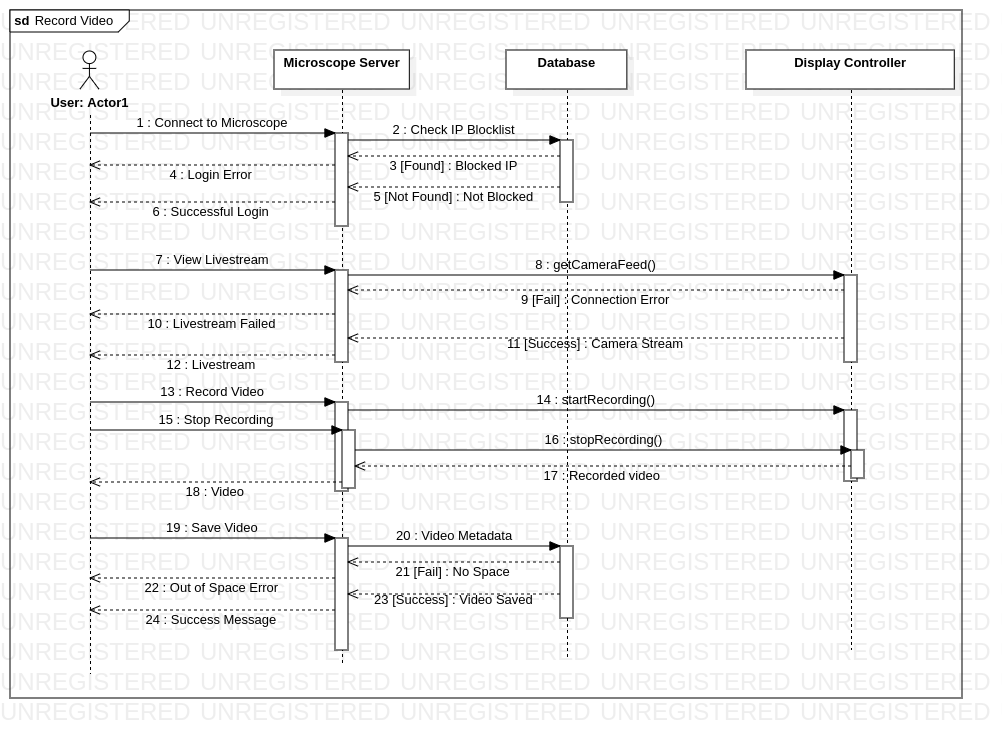
\includegraphics[scale=0.4]{Uml_Images/record_video_seq_diagram}
	\caption{Sequence Diagram of Record Video Function}
	\label{fig:record_video_seq_diagram}
\end{figure}
\begin{figure}[H]
	\centering
	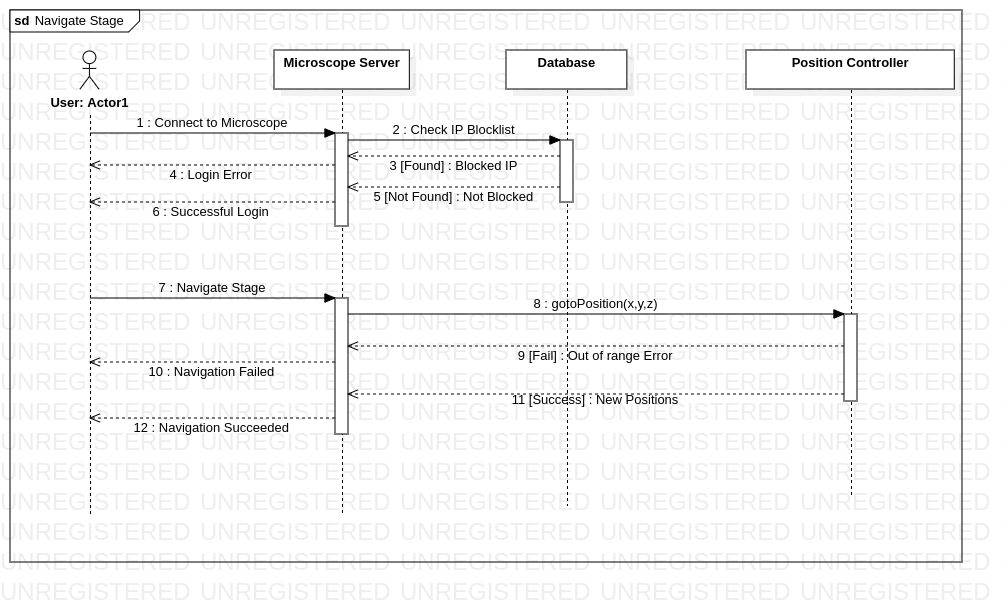
\includegraphics[scale=0.4]{Uml_Images/navigate_stage_seq_diagram}
	\caption{Sequence Diagram of Navigate Stage Function}
	\label{fig:navigate_stage_seq_diagram}
\end{figure}
\begin{figure}[H]
	\centering
	
\includegraphics[scale=0.4]{Uml_Images/block_user_seq_diagram}
	\caption{Sequence Diagram of Block User Function}
	\label{fig:block_user_seq_diagram}
\end{figure}
\begin{figure}[H]
	\centering
	
\includegraphics[scale=0.4]{Uml_Images/login_error_seq_diagram}
	\caption{Sequence Diagram of Login Error Handling}
	\label{fig:login_error_handling_seq_diagram}
\end{figure}
\begin{figure}[H]
	\centering
	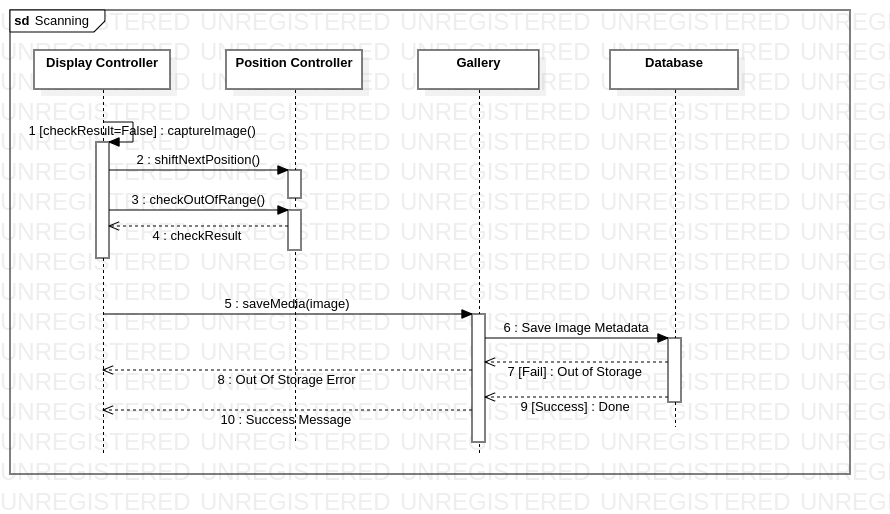
\includegraphics[scale=0.4]{Uml_Images/scanning_seq_diagram}
	\caption{Sequence Diagram of Scanning}
	\label{fig:scanning_seq_diagram}
\end{figure}
\subsubsection{Design Rationale}
Design rationales are specified where each interface is defined above.

	\begin{thebibliography}{2}
		\bibitem{ieee}
		"IEEE Standard for Information Technology--Systems Design--Software Design Descriptions," in IEEE STD 1016-2009 , vol., no., pp.1-35, 20 July 2009, doi: 10.1109/IEEESTD.2009.5167255.
		\bibitem{local} https://openflexure.gitlab.io/microscope-handbook/learn-about-the-project/local-manufacturing.html
	\end{thebibliography}

	\newpage
	
	\section{Glossary}
	\begin{table}[H]
     \centering
     \begin{tabular}{|l|p{7cm}|}
         \hline
\textbf{Admin} &
An authorized person who manages the microscope\\
\hline
\textbf{API} &
An application programming interface (API) is an interface that defines interactions between multiple software applications \\
\hline
\textbf{Command-line Interface} &
A command-line interface (CLI) processes commands to a computer program in the form of lines of text \\
\hline
\textbf{GUI} &
The graphical user interface is a form of user interface that allows users to interact with electronic devices through graphical icons and audio indicator \\
\hline
\textbf{Maintainer} & An authorized person who is responsible for keeping system software up to date and solving the technical and software-related issues in the system. \\
\hline
\textbf{Metadata} & Higher-level data that describes or annotates another data \\
\hline
\textbf{OpenFlexure Update System} & A system responsible for serving the OpenFlexure software updates to users \\
\hline
\textbf{SSH} & The Secure Shell Protocol is a cryptographic network protocol for operating network services securely over an unsecured network \\
\hline
\textbf{User} &  An unauthorized person who connects to the microscope for daily tasks\\
\hline
     \end{tabular}
     \caption{Glossary}
     \label{tab:glossary}
 \end{table}
	
	\section{Architectural Views}
	\subsection{Context View}
\subsubsection{Context Diagram}
OpenFlexure is not a part of a larger system. The communication between the OpenFlexure and Users is maintained by the OpenFlexure Web API. Users will be able to send their requests and get responses from the server using the Web API.

There are three user types in the system: Users (can be seen as end-user), Admins, and Maintainers. The system will provide different interfaces to each of them so that they can do the functions defined to them. Since Admins and Maintainers have private permissions, they will need to log in to the system using the keys defined to them to use their functions. While Admins and Maintainers will be responsible for keeping the system stable, Users will be able to use the microscope.

\begin{figure}[H]
	\centering
	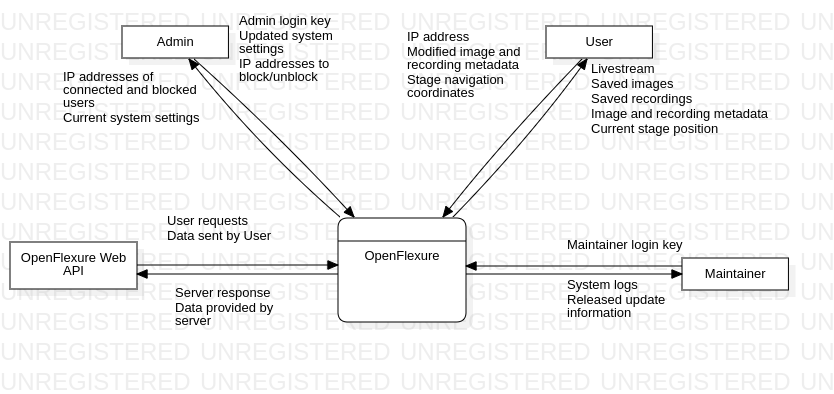
\includegraphics[scale=0.5]{Uml_Images/system_context_diagram}
	\caption{System Context Diagram for OpenFlexure}
	\label{fig:system_context_diagram}
\end{figure}


\subsubsection{Use-Case Diagram}
\begin{figure}[H]
	\centering
	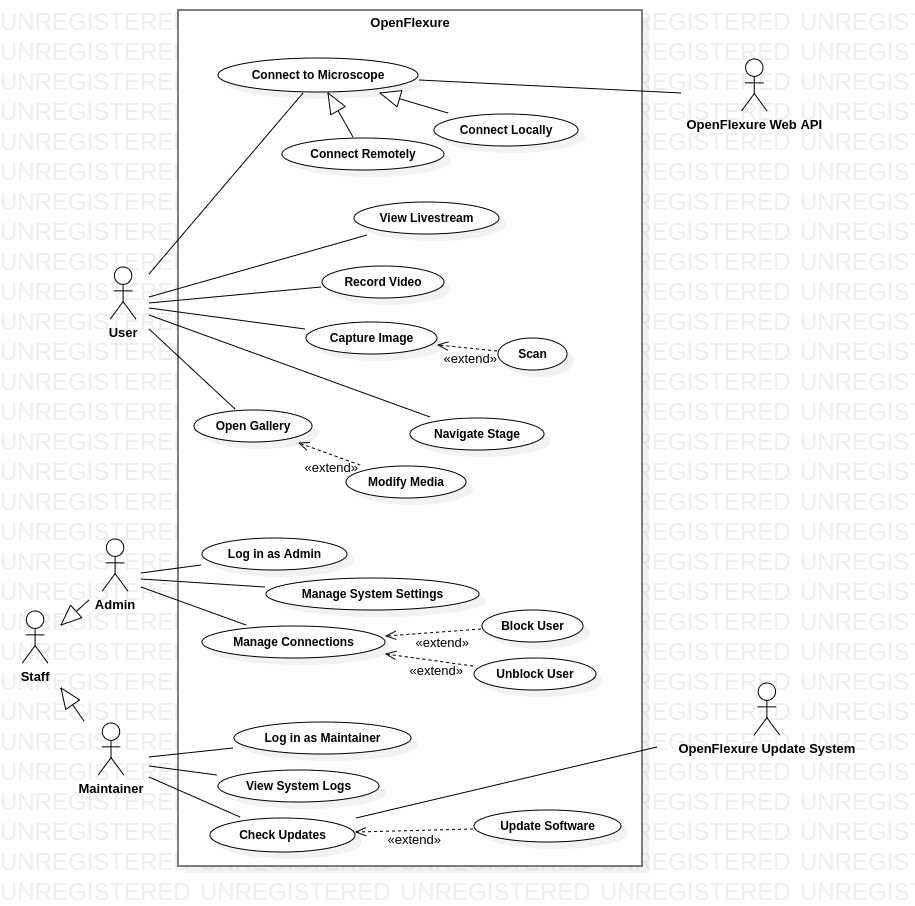
\includegraphics[scale=0.5]{Uml_Images/use_case_diagram}
	\caption{Use Case Diagram for OpenFlexure}
	\label{fig:use_case_diagram}
\end{figure}


\subsubsection{Use-Case Descriptions}
\begin{table}[H]
     \centering
     \begin{tabular}{|l|C|}
         \hline
          \textbf{Use-Case Name} & Connect to Microscope \\
         \hline
          \textbf{Actors} & User \\ 
         \hline
          \textbf{Description} & The user connects to the microscope's server. \\ 
         \hline
          \textbf{Data} & IP address of the user's computer\\ 
         \hline
          \textbf{Preconditions} & 
          Desktop application must be running. \\
         \hline
          \textbf{Stimulus} & The user clicks on "Connect to server" button placed in the home screen of the desktop application.\\ 
         \hline
          \textbf{Basic Flow} & 
          Step 1 -- The popup window contains the connection screen is opened. \newline
          Step 2 -- The user chooses "Connect remotely" option from the option boxes. \newline
          Step 3 -- Desktop application searches for the nearby microscope servers and lists the found ones. \newline
          Step 4 -- The user selects one of the microscopes listed in. \newline
          Step 5 -- The user clicks on "Connect" button. \\
         \hline
          \textbf{Alternative Flow\#1} & 
          Step 2 -- The user chooses "Connect locally" option. \newline
          Step 3 -- The desktop application searches for the web api internally stored in the Raspberry Pi, and when it finds, "Connect" button becomes available. \newline
          Step 4 -- The user clicks on "Connect" button. \\
         \hline
          \textbf{Alternative Flow\#2} & - \\
         \hline
          \textbf{Exception Flow} & If desktop application cannot found any nearby servers or the web api, the system displays an error message saying that "No device were found". If the IP address of the user is blocked, the system displays an error message saying that "Your IP address is blocked".\\
         \hline
          \textbf{Post Conditions} & The user connects to the microscope. \\ 
         \hline
     \end{tabular}
     \caption{Connect to Microscope}
     \label{tab:connect_to_microscope}
 \end{table}
\begin{table}[H]
     \centering
     \begin{tabular}{|l|C|}
         \hline
          \textbf{Use-Case Name} & View Livestream \\
         \hline
          \textbf{Actors} & User \\ 
         \hline
          \textbf{Description} & The user views the live camera feed. \\ 
         \hline
          \textbf{Data} & Camera feed\\ 
         \hline
          \textbf{Preconditions} & 
          User must be connected to the system. \newline
          Camera connection must be provided. \\
         \hline
          \textbf{Stimulus} & The user clicks on "View" button. \\ 
         \hline
          \textbf{Basic Flow} & 
          Step 1 -- The user clicks on "View" button from the side pine. \newline
		  Step 2 -- Server reaches Raspberry Pi camera. \newline
		  Step 3 -- Camera livestream is displayed in graphical user interface. \\
         \hline
          \textbf{Alternative Flow\#1} & - \\
         \hline
          \textbf{Alternative Flow\#2} & - \\
         \hline
          \textbf{Exception Flow} & If the camera connection is not established, the system displays an error message saying that "Check the camera connection".\\
         \hline
          \textbf{Post Conditions} & The livestream is displayed. \\ 
         \hline
     \end{tabular}
     \caption{View Livestream}
     \label{tab:view_livestream}
 \end{table}
\begin{table}[H]
     \centering
     \begin{tabular}{|l|C|}
         \hline
          \textbf{Use-Case Name} & Record Video \\
         \hline
          \textbf{Actors} & User, OpenFlexure Microscope \\ 
         \hline
          \textbf{Description} & The user starts recording the livestream. \\ 
         \hline
          \textbf{Data} & Recorded video\\ 
         \hline
          \textbf{Preconditions} & 
		  The user must be connected to the system. \newline
		  Camera connection must be provided. \\
         \hline
          \textbf{Stimulus} & The user clicks on "Record" button.\\ 
         \hline
          \textbf{Basic Flow} & 
          Step 1 -- The user clicks on "Record" button from the side pane. \newline
          Step 2 -- The tab that contains live camera feed and menu for recording settings opens. \newline
          Step 3 -- When user wants to start recording the livestream, he/she clicks on "Start Recording" button placed in the menu. \newline
          Step 4 -- The system sends "record" command to the "Camera System". \newline
          Step 5 -- The system displays a blinking led to indicate the recording. \newline
          Step 6 -- The user clicks on "Stop Recording" button to stop the recording. \newline
          Step 7 -- The system receives the recording from the "Camera System" and displays it in a popup window. \newline
          Step 8 -- The user gives a name to the recording by filling the textbox placed in the popup window and specifies the time interval if he/she wants to cut the recording before saving it. \newline
		  Step 9 -- The user clicks on "Save" button to save the recording. \newline
		  Step 10 -- The system saves the video to the location specified in system settings and create database record for the video using the Database Management Interface. \\
         \hline
          \textbf{Alternative Flow\#1} & 
          Step 8 -- The user clicks on the "Exit" button placed in the popup window to exit without saving the recording. \\
         \hline
          \textbf{Alternative Flow\#2} & - \\
         \hline
          \textbf{Exception Flow} & If the user tries to save the recording without naming it, the system displays an error message. If there is not enough available storage to store the recording, the system displays an error message.\\
         \hline
          \textbf{Post Conditions} & The recording is saved to the location specified in the settings and the popup window is closed. \\ 
         \hline
     \end{tabular}
     \caption{Record Video}
     \label{tab:record_video}
 \end{table}
\begin{table}[H]
     \centering
     \begin{tabular}{|l|C|}
         \hline
          \textbf{Use-Case Name} & Capture Image \\
         \hline
          \textbf{Actors} & User, OpenFlexure Microscope \\ 
         \hline
          \textbf{Description} & The user captures the image on the screen. \\ 
         \hline
          \textbf{Data} & Captured image\\ 
         \hline
          \textbf{Preconditions} & 
          The user must be connected to the system. \newline
          Camera connection must be provided. \\
         \hline
          \textbf{Stimulus} & The user clicks on "Capture" button.\\ 
         \hline
          \textbf{Basic Flow} & 
          Step 1 -- The user clicks on "Capture" button from the side pane. \newline
          Step 2 -- The tab that contains live camera feed and menu for image settings opens. \newline
          Step 3 -- When user wants to capture the image on the screen, he/she clicks on "Capture image" button placed in the menu. \newline
          Step 4 -- The system sends "capture" command to the "Camera System". \newline
          Step 5 -- The system receives the captured image from the "Camera System" and displays it in a popup window. \newline
          Step 6 -- The user gives a name to the captured image by filling the textbox placed in the popup window. \newline
		  Step 7 -- The user clicks on "Save" button to save the captured image. \newline
		  Step 8 -- The system saves the image to the location specified in system settings and create database record for the image using the Database Management Interface. \\
         \hline
          \textbf{Alternative Flow\#1} & 
          Step 6 -- The user clicks on the "Exit" button to exit without saving the captured image. \\
         \hline
          \textbf{Alternative Flow\#2} & - \\
         \hline
          \textbf{Exception Flow} & If the user tries to save the image without naming it, the system displays an error message. If there is not available storage to store the image, the system displays an error message.\\
         \hline
          \textbf{Post Conditions} & The image is saved to the location specified in the system settings and the popup window is closed. \\ 
         \hline
     \end{tabular}
     \caption{Capture Image}
     \label{tab:capture_image}
 \end{table}
\begin{table}[H]
	\centering
	\begin{tabular}{|l|C|}
		\hline
		\textbf{Use-Case Name} & Scan \\
		\hline
		\textbf{Actors} & User, OpenFlexure Microscope \\ 
		\hline
		\textbf{Description} & The system generates a scan of the area bounded by the coordinates provided by the user.\\ 
		\hline
		\textbf{Data} & Generated scan\\ 
		\hline
		\textbf{Preconditions} & 
		The user must be connected to the system. \newline
		Camera connection must be provided. \newline
		Capture tab must be opened. \\ 
		\hline
		\textbf{Stimulus} & The user clicks on "Scan" button.\\ 
		\hline
		\textbf{Basic Flow} & 
		Step 1 -- The user opens "Capture" tab from the side pane. \newline
		Step 2 -- The user activates "Scan" option by clicking the option box placed in image settings menu. \newline
		Step 3 -- The textboxes showing the coordinates that define the boundary of the area to be scanned becomes available. \newline
		Step 4 -- The user types the coordinates to the textboxes. \newline
		Step 5 -- Until the entire area has been scanned, at each step, the system sends a command to the "Motor Control System" to move by the step size specified in system settings and to the "Camera System" to capture the current image. \newline
		Step 6 -- The system merges all captured images to generate a bigger image of the area and displays it in a popup window. \newline
        Step 7 -- The user gives a name to the generated scan. \newline
		Step 8 -- The user clicks on "Save" button to save the generated scan. \newline
		Step 9 -- The system saves the scan image to the location specified in system settings and create database record for the image using the Database Management Interface. \\
		\hline
		\textbf{Alternative Flow\#1} & 
		Step 7 -- The user clicks on the "Exit" button to exit without saving the scan. \\
		\hline
		\textbf{Alternative Flow\#2} & - \\
		\hline
		\textbf{Exception Flow} & If the user tries to save the scan without naming it, the system displays an error message. If there is no available storage, the system displays an error message.\\
		\hline
		\textbf{Post Conditions} & The scan is saved to the location specified in the system settings. \\ 
		\hline
	\end{tabular}
	\caption{Scan}
	\label{tab:scan}
\end{table}
\begin{table}[H]
     \centering
     \begin{tabular}{|l|C|}
         \hline
          \textbf{Use-Case Name} & Navigate Stage \\
         \hline
          \textbf{Actors} & User, OpenFlexure Microscope \\ 
         \hline
          \textbf{Description} & The user adjusts the position of the stage. \\ 
         \hline
          \textbf{Data} & Coordinates of the stage in x, y and z axes\\ 
         \hline
          \textbf{Preconditions} & 
          User must be connected to the system. \\
         \hline
          \textbf{Stimulus} & The user clicks on "Navigate" button.\\ 
         \hline
          \textbf{Basic Flow} & 
          Step 1 -- The user clicks on "Navigate" button from the side pane. \newline
          Step 2 -- Tab that contains live camera feed and navigation menu opens. \newline
          Step 3 -- The user chooses the new x, y and z coordinates by filling the three textboxes placed in navigation menu. \newline
		  Step 4 -- The user clicks on "Apply" button. \newline
		  Step 5 -- The system sends the given coordinates to the "Motor Controller" \\
         \hline
          \textbf{Alternative Flow\#1} & - \\
         \hline
          \textbf{Alternative Flow\#2} & - \\
         \hline
          \textbf{Exception Flow} & If the motor connection is not established, the system displays an error message saying that "Check the motor connection".\\
         \hline
          \textbf{Post Conditions} & The position of the stage is physically changed. \\ 
         \hline
     \end{tabular}
     \caption{Navigate Stage}
     \label{tab:navigate_stage}
 \end{table}
\begin{table}[H]
     \centering
     \begin{tabular}{|l|C|}
         \hline
          \textbf{Use-Case Name} & Open Gallery \\
         \hline
          \textbf{Actors} & User \\ 
         \hline
          \textbf{Description} & The user displays the saved images and recorded videos. \\ 
         \hline
          \textbf{Data} & Images, recordings and metadata\\ 
         \hline
          \textbf{Preconditions} & 
          User must be connected to the system. \\
         \hline
          \textbf{Stimulus} & The user clicks on "Gallery" button \\ 
         \hline
          \textbf{Basic Flow} & 
          Step 1 -- The user clicks on "Gallery" button from the side pane. \newline
          Step 2 -- The server reaches to the database and retrieves the media records with the user's IP address in the authorIPAddress field.
          \newline
          Step 3 -- The system displays a list of images and recordings in a new tab as a grid style gallery where each entry has thumbnail and metadata of the corresponding media. \\
         \hline
          \textbf{Alternative Flow\#1} &  - \\ 
         \hline
          \textbf{Alternative Flow\#2} & -\\
         \hline
          \textbf{Exception Flow} & If there is no saved media associated with the user, the system displays a message saying that "No saved media were found."\\
         \hline
          \textbf{Post Conditions} & The user views the media saved by him/her. \\ 
         \hline
     \end{tabular}
     \caption{Open Gallery}
     \label{tab:open_gallery}
 \end{table}
\begin{table}[H]
     \centering
     \begin{tabular}{|l|C|}
         \hline
          \textbf{Use-Case Name} & Modify Media \\
         \hline
          \textbf{Actors} & User \\ 
         \hline
          \textbf{Description} & The user modifies the saved media. \\ 
         \hline
          \textbf{Data} & Metadata of the saved images and recordings\\ 
         \hline
          \textbf{Preconditions} & 
          User must be connected to the system. \newline
          Gallery tab must be active \\
         \hline
          \textbf{Stimulus} & The user clicks on one of the media entries in the gallery. \\ 
         \hline
          \textbf{Basic Flow} & 
          Step 1 --  The user clicks the media entry he/she wants to modify in the gallery. \newline
          Step 2 -- The popup window contains metadata information of the clicked media opens. \newline
          Step 3 -- The user changes the metadata of the media. \newline
          Step 4 -- The user clicks on "Save" button to save the updated metadata. \newline
          Step 5 -- The system updates the corresponding database records using the Database Management Interface. \\
         \hline
          \textbf{Alternative Flow\#1} &            
          Step 3 -- The user clicks on "Delete" button. \newline
          Step 4 -- The media is deleted from the storage location and corresponding database records is deleted from the database. \\
         \hline
          \textbf{Alternative Flow\#2} & -\\
         \hline
          \textbf{Exception Flow} & - \\
         \hline
          \textbf{Post Conditions} & The media is either deleted or its metadata is updated. \\ 
         \hline
     \end{tabular}
     \caption{Modify Media}
     \label{tab:modify_media}
 \end{table}
\begin{table}[H]
     \centering
     \begin{tabular}{|l|C|}
         \hline
          \textbf{Use-Case Name} & Log in as Admin \\
         \hline
          \textbf{Actors} & Admin \\ 
         \hline
          \textbf{Description} & The admin connects to server with his/her login key.\\ 
         \hline
          \textbf{Data} & Admin login key\\ 
         \hline
          \textbf{Preconditions} & - \\
         \hline
          \textbf{Stimulus} & The admin sends login request to server using the terminal.\\ 
         \hline
          \textbf{Basic Flow} & 
          Step 1 -- The server receives the login request. \newline
          Step 2 -- The server asks for the admin login key. \newline
          Step 3 -- Maintainer types his/her login key to the terminal. \newline
          Step 4 -- The system reaches to the local database and verifies the given login key.   \newline
          Step 5 -- The system signs in the admin. \\
         \hline
          \textbf{Alternative Flow\#1} & - \\
         \hline
          \textbf{Alternative Flow\#2} & - \\
         \hline
          \textbf{Exception Flow} & If the given key is invalid, the system displays an error message saying that "Given key is invalid". The system saves the report of the failed login attempt and the IP address of the user to the system logs. Then, the flow starts again from Step 2. \\
         \hline
          \textbf{Post Conditions} & The admin command line interface opens. \\ 
         \hline
     \end{tabular}
     \caption{Log in as Admin}
     \label{tab:log_in_as_admin}
 \end{table}
\begin{table}[H]
     \centering
     \begin{tabular}{|l|C|}
         \hline
          \textbf{Use-Case Name} & Manage System Settings \\
         \hline
          \textbf{Actors} & Admin \\ 
         \hline
          \textbf{Description} & The admin manages and updates the system settings. \\ 
         \hline
          \textbf{Data} & Current settings, updated setting\\ 
         \hline
          \textbf{Preconditions} & 
		  The admin must be logged in. \\
         \hline
          \textbf{Stimulus} & The admin gives "manage settings" command using the admin command line interface. \\ 
         \hline
          \textbf{Basic Flow} & 
          Step 1 -- The system reaches to the local database and retrieve the system settings record. \newline    
          Step 2 -- The system displays the current settings as a table where each row consists of the setting name and current value of the setting. \newline
          Step 3 -- The admin gives "set \{setting name\} \{new value\}" command to change the value of the specified setting. \newline
          Step 4 -- The system reaches to database and changes the value of the given settings field. \\
         \hline
          \textbf{Alternative Flow\#1} &  - \\
         \hline
          \textbf{Alternative Flow\#2} & -\\
         \hline
          \textbf{Exception Flow} & - \\
         \hline
          \textbf{Post Conditions} & The system settings are updated. \\ 
         \hline
     \end{tabular}
     \caption{Manage System Settings}
     \label{tab:manage_system_settings}
 \end{table}
\begin{table}[H]
     \centering
     \begin{tabular}{|l|C|}
         \hline
          \textbf{Use-Case Name} & Manage Connections \\
         \hline
          \textbf{Actors} & Admin \\ 
         \hline
          \textbf{Description} & The admin views the list of connected and blocked users. \\ 
         \hline
          \textbf{Data} & IP addresses, types (user, maintainer or admin) and the statuses (connected, blocked) of the users. \\
         \hline
          \textbf{Preconditions} & 
          The admin must be logged in. \\
         \hline
          \textbf{Stimulus} & The admin gives "manage connections" command using the admin command-line interface.\\ 
         \hline
          \textbf{Basic Flow} & 
          Step 1 -- The system reaches to the database and gathers records of the connected and blocked users. \newline
          Step 2 -- The system displays the list of IP addresses, connection times and the statuses (connected, blocked) of the users. \\
         \hline
          \textbf{Alternative Flow\#1} & -\\
         \hline
          \textbf{Alternative Flow\#2} & - \\
         \hline
          \textbf{Exception Flow} & If there is no connected or blocked user, the system displays an error message saying that "No data were found".\\
         \hline
          \textbf{Post Conditions} & The admin views the connected and blocked users. \\ 
         \hline
     \end{tabular}
     \caption{Manage Connections}
     \label{tab:manage_connections}
 \end{table}
\begin{table}[H]
     \centering
     \begin{tabular}{|l|C|}
         \hline
          \textbf{Use-Case Name} & Block User \\
         \hline
          \textbf{Actors} & Admin \\ 
         \hline
          \textbf{Description} & The admin blocks a user with given IP address. \\ 
         \hline
          \textbf{Data} & IP address of the user\\ 
         \hline
          \textbf{Preconditions} & 
          The admin must be logged in. \newline
          The admin must have given the "manage connections" command beforehand.\\
         \hline
          \textbf{Stimulus} & The admin types "block user" command in the admin command-line interface.\\ 
         \hline
          \textbf{Basic Flow} & 
          Step 1 -- The system asks for the IP address of the user to block. \newline
          Step 2 -- The admin gives the IP address of the user obtained from the list displayed after "manage connections" command. \newline
          Step 3 -- Server reaches to the database and sets the blockStatus field of the user record with the given IP Address as "blocked" \\
         \hline
          \textbf{Alternative Flow\#1} & -\\
         \hline
          \textbf{Alternative Flow\#2} & - \\
         \hline
          \textbf{Exception Flow} & If there is no connected user with the given IP address, the system displays an error message saying that "Invalid Ip address". If the user with the given IP address  has already been blocked, the system displays an error message saying that "The given IP address has already been blocked".\\
         \hline
          \textbf{Post Conditions} & The user with the given IP address will not be able to connect to the server until it is unblocked.\\ 
         \hline
     \end{tabular}
     \caption{Block User}
     \label{tab:block_user}
 \end{table}
\begin{table}[H]
     \centering
     \begin{tabular}{|l|C|}
         \hline
          \textbf{Use-Case Name} & Unblock User \\
         \hline
          \textbf{Actors} & Admin \\ 
         \hline
          \textbf{Description} & The admin unblocks a user with given IP address. \\ 
         \hline
          \textbf{Data} & IP address of the user\\ 
         \hline
          \textbf{Preconditions} & 
          The admin must be logged in. \newline
          The admin must have given the "manage connections" command beforehand.\\
         \hline
          \textbf{Stimulus} & The admin types "unblock user" command in the admin command-line interface.\\ 
         \hline
          \textbf{Basic Flow} & 
          Step 1 -- The system asks for the IP address of the user to unblock. \newline
          Step 2 -- The admin gives the IP address of the user obtained from the list displayed after "manage connections" command. \newline
          Step 3 -- Server reaches to the database and sets the blockStatus field of the user record with the given IP Address as "unblocked" \\
         \hline
          \textbf{Alternative Flow\#1} & -\\
         \hline
          \textbf{Alternative Flow\#2} & - \\
         \hline
          \textbf{Exception Flow} & If there is no blocked user with the given IP address, the system displays an error message saying that "No blocked users were found". \\
         \hline
          \textbf{Post Conditions} & The user with the given IP address will be able to connect to the server again. \\ 
         \hline
     \end{tabular}
     \caption{Unblock User}
     \label{tab:unblock_user}
 \end{table}
\begin{table}[H]
     \centering
     \begin{tabular}{|l|C|}
         \hline
          \textbf{Use-Case Name} & Log in as Maintainer \\
         \hline
          \textbf{Actors} & Maintainer \\ 
         \hline
          \textbf{Description} & The maintainer connects to server with his/her login key.\\ 
         \hline
          \textbf{Data} & Maintainer login key\\ 
         \hline
          \textbf{Preconditions} & - \\
         \hline
          \textbf{Stimulus} & The maintainer sends login request to server from the terminal.\\ 
         \hline
          \textbf{Basic Flow} & 
          Step 1 -- The server receives the login request. \newline
          Step 2 -- The server asks for the maintainer login key. \newline
          Step 3 -- Maintainer types his/her login key to the terminal. \newline
          Step 4 -- The system reaches to the local database and verifies the given login key.   \newline
          Step 5 -- The system signs in the maintainer. \\
         \hline
          \textbf{Alternative Flow\#1} & - \\
         \hline
          \textbf{Alternative Flow\#2} & - \\
         \hline
          \textbf{Exception Flow} & If the given key is invalid, the system displays an error message saying that "Given key is invalid". The system saves the log of the failed login attempt and the IP address of the user to the database. Then, the flow starts again from Step 2. \\
         \hline
          \textbf{Post Conditions} & The maintainer command-line interface opens. \\ 
         \hline
     \end{tabular}
     \caption{Log in as Maintainer}
     \label{tab:log_in_as_maintainer}
 \end{table}
\begin{table}[H]
     \centering
     \begin{tabular}{|l|C|}
         \hline
          \textbf{Use-Case Name} & View system logs \\
         \hline
          \textbf{Actors} & Maintainer \\ 
         \hline
          \textbf{Description} & The maintainer can list and view the system logs sorted by their dates.\\ 
         \hline
          \textbf{Data} & System logs\\ 
         \hline
          \textbf{Preconditions} & 
          Maintainer must be logged in. \\
         \hline
          \textbf{Stimulus} & The maintainer gives "view logs" command using the command-line interface.\\ 
         \hline
          \textbf{Basic Flow} & 
          Step 1 -- The server takes the request. \newline
          Step 2 -- The server gathers the system logs from the database. \newline
          Step 3 -- The system displays the system logs in command-line interface. \\
         \hline
          \textbf{Alternative Flow\#1} & - \\
         \hline
          \textbf{Alternative Flow\#2} & - \\
         \hline
          \textbf{Exception Flow} & If there is no system logs in database, the system displays a message saying that "No system logs were found". \\
         \hline
          \textbf{Post Conditions} & The system logs are displayed in the maintainer's interface. \\ 
         \hline
     \end{tabular}
     \caption{View System Logs}
     \label{tab:view_system_logs}
 \end{table}
\begin{table}[H]
     \centering
     \begin{tabular}{|l|C|}
         \hline
          \textbf{Use-Case Name} & Check Updates \\
         \hline
          \textbf{Actors} & Maintainer, OpenFlexure Update System \\ 
         \hline
          \textbf{Description} & The maintainer checks for the software updates.\\ 
         \hline
          \textbf{Data} & System's current software version, released update information\\
         \hline
          \textbf{Preconditions} & 
          Maintainer must be logged in. \\
         \hline
          \textbf{Stimulus} & The maintainer gives "check updates" command using the command line interface.\\ 
         \hline
          \textbf{Basic Flow} & 
          Step 1 -- The server retrieves the version number of the software from the database. \newline
          Step 2 -- The server sends the current version number of the software to the OpenFlexure Update System. \newline
          Step 3 -- The server receives the information about the latest update returned by the OpenFlexure Update System. \newline
          Step 4 -- The server displays the version number, size, release date and changelog of the update in command-line interface. \\
         \hline
          \textbf{Alternative Flow\#1} & - \\
         \hline
          \textbf{Alternative Flow\#2} & - \\
         \hline
          \textbf{Exception Flow} & If the system is already using the latest version, an error message saying that "No updates were found" is displayed. \\
         \hline
          \textbf{Post Conditions} & Information about the latest update is displayed in the command-line interface. \\ 
         \hline
     \end{tabular}
     \caption{Check Updates}
     \label{tab:check_updates}
 \end{table}
\begin{table}[H]
     \centering
     \begin{tabular}{|l|C|}
         \hline
          \textbf{Use-Case Name} & Update Software \\
         \hline
          \textbf{Actors} & Maintainer, OpenFlexure Update System \\ 
         \hline
          \textbf{Description} & The maintainer updates the system software.\\ 
         \hline
          \textbf{Data} & Installable update package\\ 
         \hline
          \textbf{Preconditions} & 
          Maintainer must be logged in. \newline
          Maintainer must have given the "check updates" command beforehand.\\
         \hline
          \textbf{Stimulus} & The maintainer gives "update" command using the command line interface.\\ 
         \hline
          \textbf{Basic Flow} & 
          Step 1 -- The server requests the update package from the OpenFlexure Update System. \newline
          Step 2 -- The package is downloaded to the Raspberry Pi. \newline
          Step 3 -- The server installs the downloaded package. \newline
          Step 4 -- The server saves the version number and the release date of the update to the corresponding database table. \\
         \hline
          \textbf{Alternative Flow\#1} & - \\
         \hline
          \textbf{Alternative Flow\#2} & - \\
         \hline
          \textbf{Exception Flow} & If an error is encountered during the installation, for example, if the downloaded package is corrupted, the system saves the detailed error log into the database. \\
         \hline
          \textbf{Post Conditions} & The system is updated to the latest version. \\ 
         \hline
     \end{tabular}
     \caption{Update Software}
     \label{tab:update_software}
 \end{table}

\subsection{Composition View}
The Composition View section provides information about the components of the system. Detailed information can be found corresponding parts of the section.
\subsubsection{Component Diagram}
\begin{figure}[H]
	\centering
	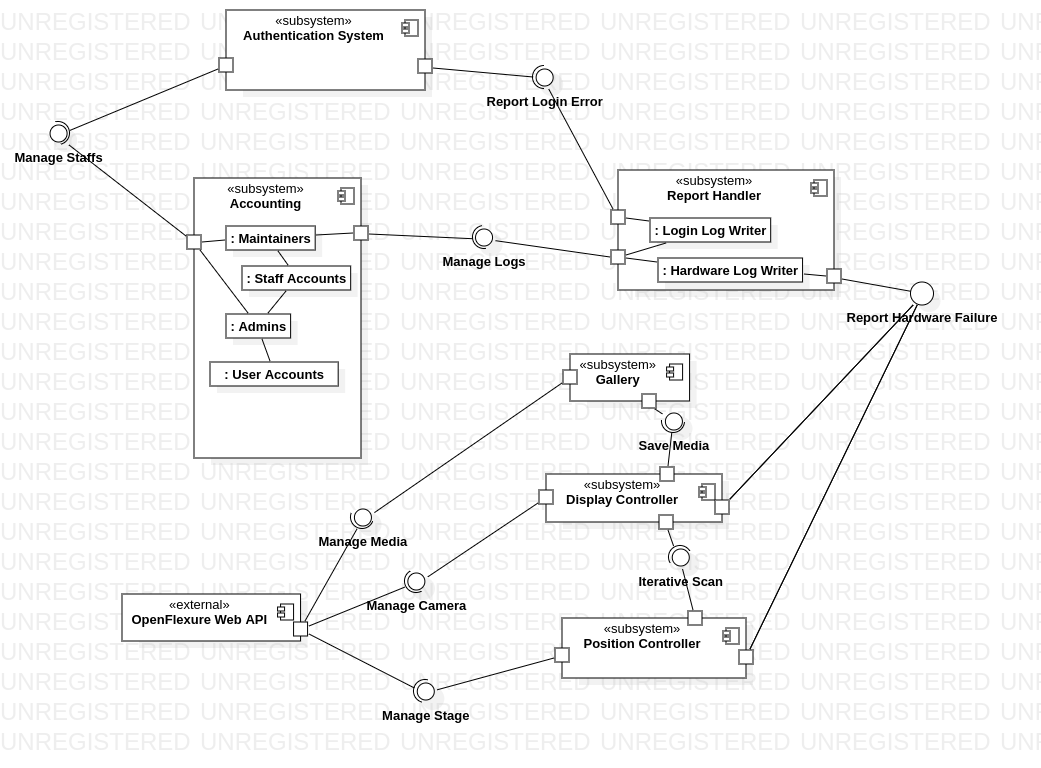
\includegraphics[scale=0.4]{Uml_Images/component_diagram}
	\caption{Component Diagram for OpenFlexure}
	\label{fig:component_diagram}
\end{figure}

\subsubsection{Deployment Diagram}
\begin{figure}[H]
	\centering
	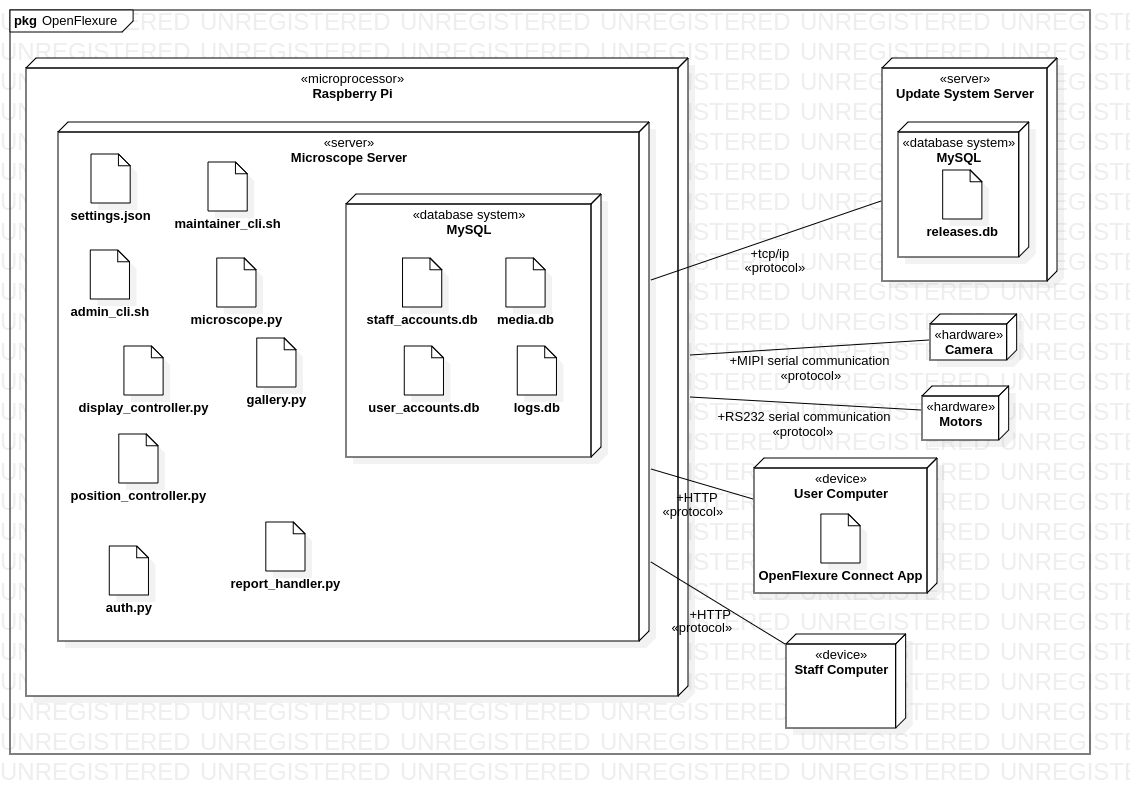
\includegraphics[scale=0.4]{Uml_Images/deployment_diagram}
	\caption{Deployment Diagram for OpenFlexure}
	\label{fig:deployment_diagram}
\end{figure}

\subsubsection{Design Rationale}
\paragraph{Component Diagram}
\begin{itemize}
	\item To allow the admins to use Block User and Unblock User functions defined in use-case diagram, Admins part is associated with the User Accounts part.
	\item To allow the admins to use Block User and Unblock User functions defined in use-case diagram, Admins part is associated with the User Accounts part.
	\item To allow the Authentication Systems to check the provided password information, Accounting provides an interface.
	\item Report Handler provides two different interfaces which are used by the Authentication System, Position Controller and Display Controller to write and store Login related and Hardware related issues.
	\item To be able to store the media (images and videos) generated by the Display Controller, Gallery provides an interface.
\end{itemize}
\paragraph{Deployment Diagram}
\begin{itemize}
	\item MySQL is used as database management system to store System Logs, Staff Accounts, User Connection Records and saved Media Metadata.
	\item System Settings are stored in json file, since it is easier and faster to process json file.
	\item To provide Admin Commmand-line Interface and Maintainer Command-line Interface two bash programs are stored in the server, admin\_cli.sh and maintainer\_cli.sh, respectively.
	\item Authentications of the staff personal are done by auth.py
	\item For Raspberry PI Camera hardware and Motor hardware MIPI and RS232 serial communication protocols are used.
\end{itemize}

\subsection{Information View}
The Information View section contains information about the organization and the relations of the data stored in the system.
\subsubsection{Class Diagram}

\begin{figure}[H]
	\centering
	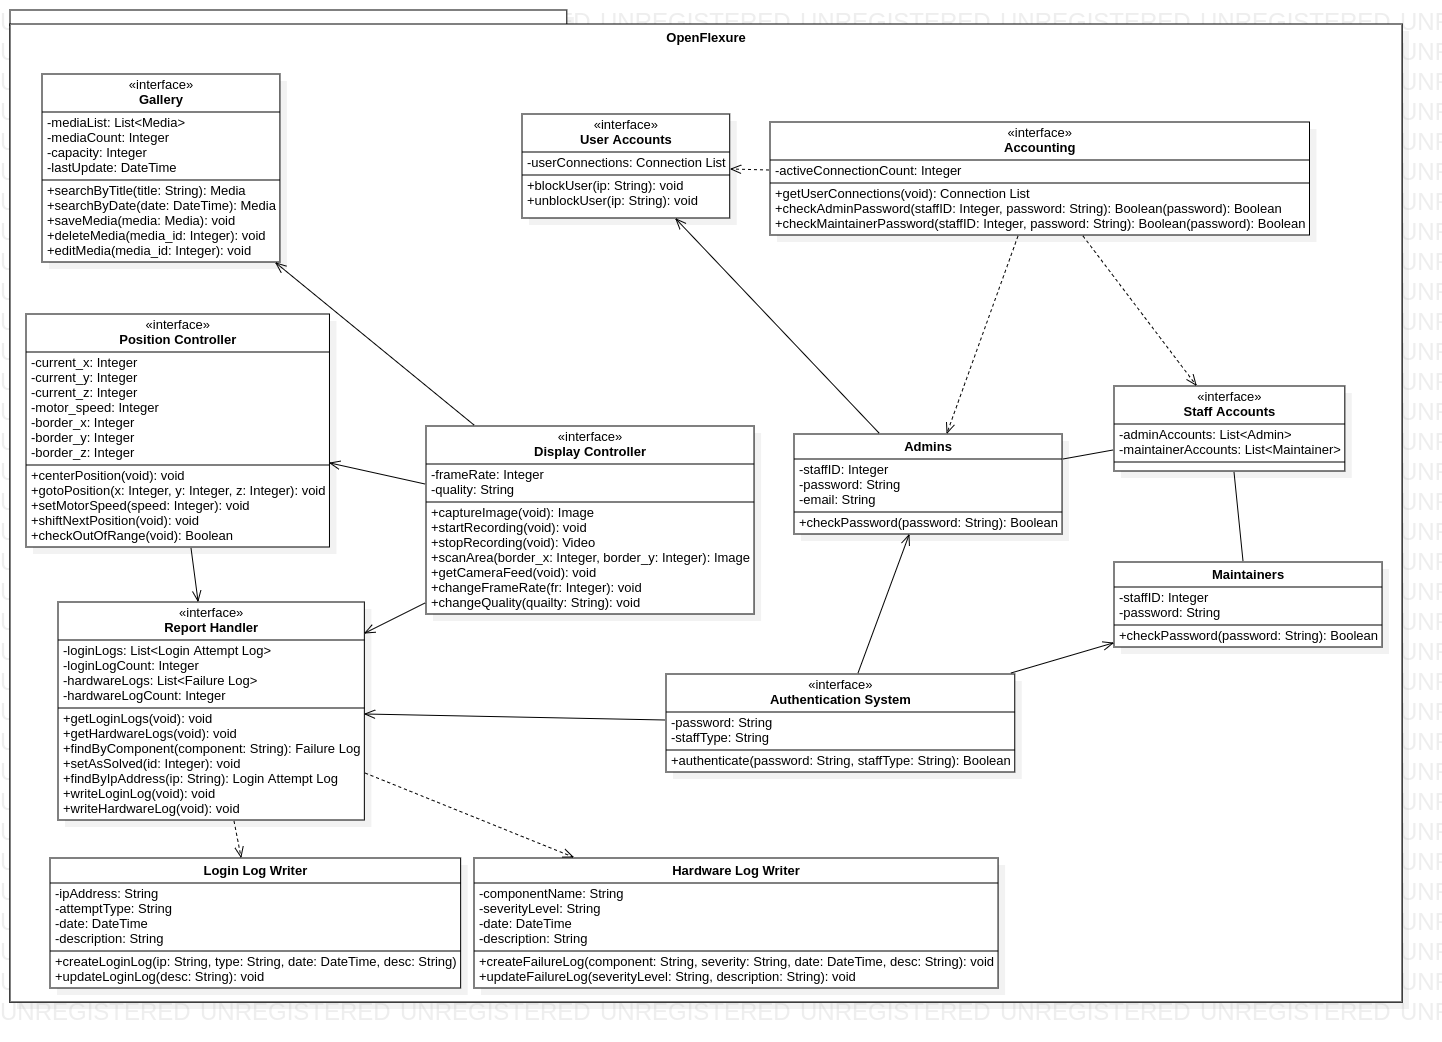
\includegraphics[scale=0.3]{Uml_Images/interface_class_diagram}
	\caption{Interface Class Diagram for OpenFlexure}
	\label{fig:interface_class_diagram}
\end{figure}

\begin{table}[H]
	\centering
	\begin{tabular}{|l|C|}
		\hline
		\textbf{Operation}   &  \textbf{Description}\\
		\hline
		searchByTitle   &  returns the media with given title\\
		\hline
		searchByDate   &  returns the media with given date\\
		\hline
		saveMedia  &  saves the given media to the gallery media list\\
		\hline
		deleteMedia   &  delete the media with given id from the gallery media list\\
		\hline
		editMedia   &  edits the media with given id\\
		\hline
		centerPosition   &  positions the stage to the center\\
		\hline
		gotoPosition   &  positions the stage to the point with the given coordinates\\
		\hline
		setMotorSpeed  &  sets the motor speed\\
		\hline
		shiftNextPosition  &  shifts the stage position to the next one by incrementing the current coordinates\\
		\hline
		checkOutOfRange  &  checks if the current coordinates are out of range\\
		\hline
		captureImage  &  captures the displayed livestream and returns the captured image\\
		\hline
		startRecording   &  starts recording the livestream\\
		\hline
		stopRecording   &  stops the ongoing recording and returns the recorded video\\
		\hline
		scanArea & scans the area with the given border coordinates and returns it as image\\
		\hline
		getCameraFeed & streams the live camera feed \\
		\hline
		changeFrameRate & changes the frame rate of the camera\\
		\hline
		changeQuality & changes the quality of the camera\\
		\hline
		getLoginLogs & returns the list of Login Attempt Logs\\
		\hline
		getHardwareLogs & returns the list of Failure Logs\\
\hline
		findByComponent & returns the Failure Log with the given component name\\
\hline
		setAsSolved & sets the status of the log with given id as solved\\
\hline
		findByIpAddress & returns the Login Attempt Log with the given component name\\
\hline
		writeLoginLog & writes the login log created by Login Log Writer to the loginLogs list\\
\hline
		writeHardwareLog & writes the hardware log created by Hardware Log Writer to the hardwareLogs list\\
\hline
		createLoginLog & creates a Login Attempt Log and fills it with the given parameters\\
\hline
	\end{tabular}
\end{table}

\begin{table}[H]
	\centering
	\begin{tabular}{|l|C|}
		\hline
	updateLoginLog & updates the Login Attempt Log with the given id\\
	\hline
	createFailureLog & creates a Failure Log and fills it with the given parameters\\
	\hline
	updateFailureLog & updates the Failure Log with the given id\\
	\hline
	authenticate & checks the password of the user with given staff type and authenticates him/her\\
	\hline
	getUserConnections & returns the list of Connections \\
	\hline
	checkAdminPassword & compares the given password with the password of the admin with given staffID and returns the result of the comparison \\
	\hline
	checkMaintainerPassword & compares the given password with the password of the maintainer with given staffID and returns the result of the comparison \\
	\hline
	blockUser & sets the blockStatus of the user with the given ip as True \\
	\hline
	unblockUser & sets the blockStatus of the user with the given ip as False \\
	\hline
	checkPassword & compares the given password with the password of the admin/maintainer \\
	\hline
	\end{tabular}
	\caption{Operation Descriptions}
	\label{tab:operation_descriptions}
\end{table}

\begin{figure}[H]
	\centering
	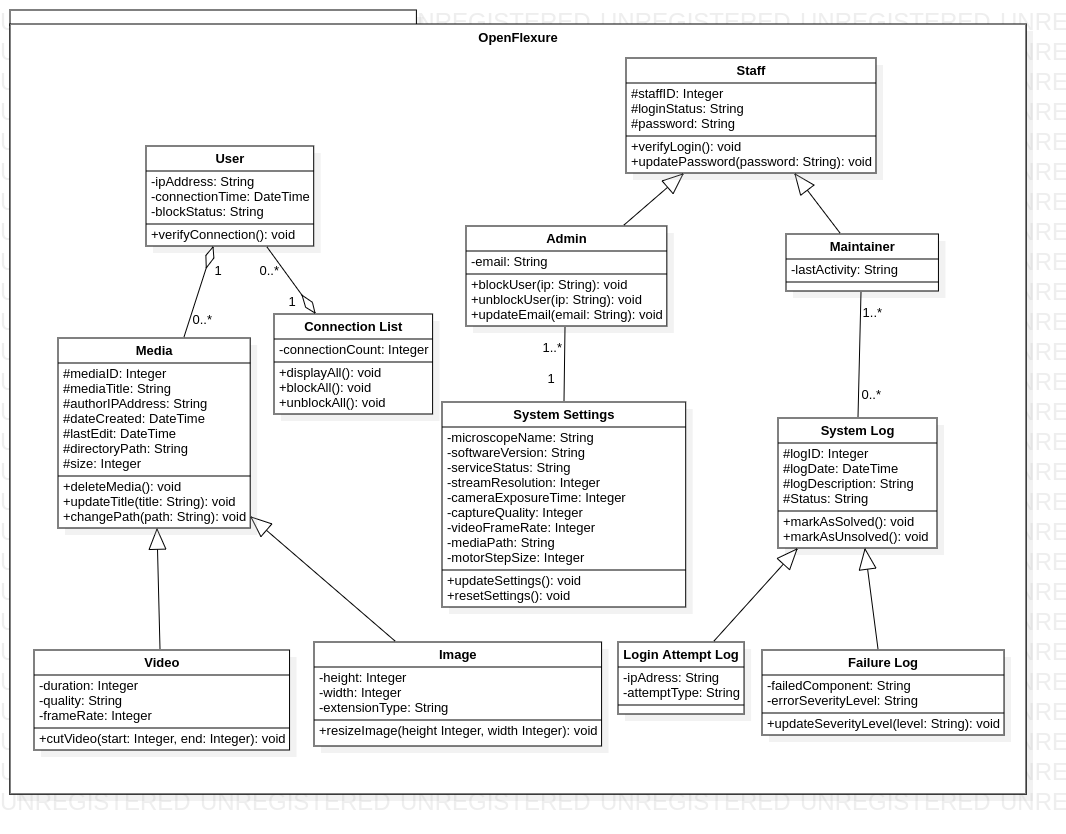
\includegraphics[scale=0.4]{Uml_Images/db_class_diagram}
	\caption{Database Class Diagram for OpenFlexure}
	\label{fig:db_class_diagram}
\end{figure}

\subsubsection{Database Operations}
\begin{table}[H]
	\centering
	\begin{tabular}{|p{5cm}|p{7cm}|}
		\hline
		\textbf{Operation} & \textbf{CRUD Operations} \\
		\hline
		verifyLogin &
		CREATE:\newline
		READ: \texttt{Staff} \newline
		UPDATE: \texttt{Staff} \newline
		DELETE: \\
		\hline
		updatePassword &
		CREATE:\newline
		READ: \newline
		UPDATE: \texttt{Staff}\newline
		DELETE: \\
		\hline
		updateEmail &
		CREATE:\newline
		READ: \newline
		UPDATE: \texttt{Admin}\newline
		DELETE: \\
		\hline
		blockUser &
		CREATE:\newline
		READ: \newline
		UPDATE: \texttt{User}\newline
		DELETE: \\
		\hline
		unblockUser &
		CREATE:\newline
		READ: \newline
		UPDATE: \texttt{User}\newline
		DELETE: \\
		\hline
		updateSettings &
		CREATE:\newline
		READ: \newline
		UPDATE: \texttt{Settings}\newline
		DELETE: \\
		\hline
		resetSettings &
		CREATE:\newline
		READ: \texttt{Settings}\newline
		UPDATE: \texttt{Settings}\newline
		DELETE: \\
		\hline
		markAsSolved &
		CREATE:\newline
		READ: \newline
		UPDATE: \texttt{System Log}\newline
		DELETE: \\
		\hline
	\end{tabular}
\end{table}

\begin{table}[H]
	\centering
	\begin{tabular}{|p{5cm}|p{7cm}|}
		\hline
		markAsUnsolved &
		CREATE:\newline
		READ: \newline
		UPDATE: \texttt{System Log}\newline
		DELETE: \\
		\hline
		updateSeverityLevel &
		CREATE:\newline
		READ: \newline
		UPDATE: \texttt{Failure Log}\newline
		DELETE: \\
		\hline
		verifyConnection &
		CREATE: \newline
		READ: \texttt{User}\newline
		UPDATE: \texttt{User}\newline
		DELETE: \\
		\hline
		deleteMedia &
		CREATE: \newline
		READ:  \newline
		UPDATE: \newline
		DELETE: \texttt{Media} \\
		\hline
		updateTitle &
		CREATE: \newline
		READ:  \newline
		UPDATE: \texttt{Media} \newline
		DELETE:  \\
		\hline
		changePath &
		CREATE: \newline
		READ:  \newline
		UPDATE: \texttt{Media} \newline
		DELETE:  \\
		\hline
		cutVideo &
		CREATE: \newline
		READ:  \newline
		UPDATE: \texttt{Video} \newline
		DELETE:  \\
		\hline
		resizeImage &
		CREATE: \newline
		READ:  \newline
		UPDATE: \texttt{Image} \newline
		DELETE:  \\
		\hline
		displayAll &
		CREATE: \newline
		READ: \texttt{Connection List}, \texttt{User}\newline
		UPDATE: \newline
		DELETE: \\
		\hline
	\end{tabular}
\end{table}
\begin{table}[H]
	\centering
	\begin{tabular}{|p{5cm}|p{7cm}|}
		\hline
		blockAll &
		CREATE: \newline
		READ: \texttt{Connection List} \newline
		UPDATE: \texttt{User} \newline
		DELETE: \\
		\hline
		unblockAll &
		CREATE: \newline
		READ: \texttt{Connection List} \newline
		UPDATE: \texttt{User} \newline
		DELETE: \\
		\hline
	\end{tabular}
	\caption{CRUD Operations}
	\label{tab:crud_operations}
\end{table}

\subsubsection{Design Rationale}
\paragraph{Interface Class Diagram}
\begin{itemize}
	\item Report Handler is responsible for creating and storing logs related to hardware failures and login errors.
	\item Both Display Controller and Position Controller associated with the Report Handler to report hardware related problems.
	\item Authentication System is associated with the Report Handler to report suspicious login attempts.
	\item To allow the maintainers to use View System Logs function defined in use-case diagram, Maintainers component uses the interface provided by the Report Handler.
	\item To allow the admins to use Block User and Unblock User functions defined in use-case diagram, Admins part is associated with the User Accounts part.
	\item To be able to store the captured images, scans and recorded videos, Display Controller is associated with the Gallery.
\end{itemize}
\paragraph{Database Class Diagram}
\begin{itemize}
	\item For easy and fast usability of the microscope, users do not have to authenticate to the system. Therefore, for user records, password information is omitted.
	\item To avoid repetition of the attributes, Media, System Log and Staff parent classes are defined. 
	\item To be able to handle different types of errors, Login Attempt Log and Failure Log classes are created.
	\item To allow the maintainer to use View System Logs function defined in use-case diagram, Maintainer and System Logs classes are linked to each other.
\end{itemize}

\subsection{Interface View}
The Interface View section provides information about the internal and external interfaces of the system.
\subsubsection{Internal Interfaces}
\paragraph{Interface between Accounting and Authentication System}
The interface provided by Accounting component is used by the Authentication System to verify the provided staffID and password.
\subparagraph{Design Rationale:}
\begin{itemize}
	\item Authentication System sends the given staffID and password parameters to the Accounting component.
	\item Based on the type of the staff Accounting checks the password using checkPassword operation belongs to either Admins or Maintainers parts.
	\item Returns the result of the checkPassword operation.
\end{itemize}
\paragraph{Interface between Authentication System and Report Handler}
The interface provided by the Report Handler is used by the Authentication System to report suspicious and wrong login attempts.
\subparagraph{Design Rationale:}
\begin{itemize}
	\item If the boolean result returned by the Accounting, Authentication System sends the provided information to the Report Handler.
	\item Report Handler saves the Login Attempt Log created by the Login Log Writer part in the loginLogs list. 
\end{itemize}
\paragraph{Interface between Accounting and Report Handler}
The interface provided by the Report Handler is used by the Accounting and especially its subcomponent Maintainers to display and check the written System Logs.
\subparagraph{Design Rationale:}
\begin{itemize}
	\item Report Handler provides the loginLogs list and hardwareLogs list to the Accounting and specifically Maintainers part to allow maintainers to use View System Logs function.
\end{itemize}
\paragraph{Interface between Report Handler and Display Controller and Position Controller}
The interface provided by the Report Handler is used by both Display and Position Controllers to report any hardware related technical issues.
\subparagraph{Design Rationale:}
\begin{itemize}
	\item Since Display and Position Controllers are related to hardware devices (camera and motors), it is possible to have hardware related issues. This interface is for handling the hardware related problems.
	\item Report Handler saves the Failure Log created by the Hardware Log Writer part in the hardwareLogs list. 
\end{itemize}
\paragraph{Interface between Display Controller and Position Controller}
The interface provided by the Position Controller is used by the Display Controller for the scanArea operation. In this operation by using this interface Display Controller is able to iteratively move the camera position to scan the area.
\subparagraph{Design Rationale:}
\begin{itemize}
	\item To be able to use Scan function defined in the use-case diagram Display Controller serves scanArea function.
	\item To use the scanArea function position of the stage should be shifted iteratively. Position Controller serves this interface to allow Display Controller to shift stage position in each iteration.
\end{itemize}
\paragraph{Interface between Display Controller and Gallery}
The interface provided by the Gallery is used by the Display Controller to save the captured Images, scans, recorded videos.
\subparagraph{Design Rationale:}
\begin{itemize}
	\item Display Controller is responsible to implement Capture Image, Record Video and Scan functions defined in use-case diagram.
	\item To be able to store the media generated by the Display Controller, Gallery serves this interface.
\end{itemize}
\subsubsection{External Interfaces}
	\paragraph{User Interfaces}
	\begin{itemize}
		\item \textbf{User Web Interface} \\
		Users use a web interface written in javascript using Vue.js framework which is running inside the local microscope server. User can reach to  the User Web Interface by just typing the ip address and designated port of the microscope's server in their browser. Users are able to control the microscope and view the camera feed using the user interface. User Web Interface provides live stream camera feed, navigation menu to change the position of the stage and gallery to view and update the saved media. \\
		\textbf{Design Rationale:} 
		\begin{enumerate}
			\item User web interface has a very simple design to allow inexperienced users to use the provided features easily.
			\item It has a help window that contains solutions for the frequently faced problems to guide users faced with such problems.
			\item The icons have been placed inside the tab buttons in addition to button labels to ensure that the desired feature can be found easily.
		\end{enumerate}
		\begin{figure}[H]
			\centering
			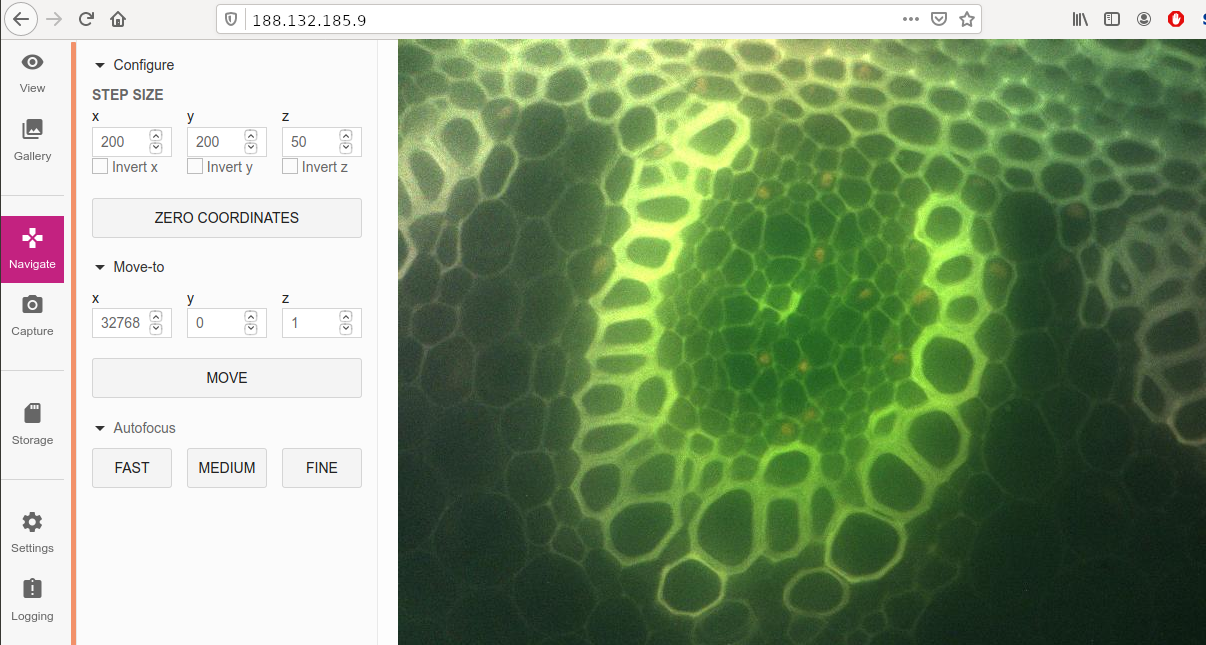
\includegraphics[scale=0.3]{Figures/user_web_interface}
			\caption{OpenFlexure User Web Interface}
			\label{fig:user_web_interface}
		\end{figure}
		\item \textbf{Admin Command-line Interface} \\
		System administrators use a command-line interface to manage the system. Administrators are able to list the detailed information about connected/blocked users such as User IPs, block/unblock status, and connection time. Using the commands provided by this interface, the administrators can view/manage/update system settings and block/unblock users. Admin command-line interface is provided by a bash script placed inside the local microscope server and starts to run when an admin connects to the microscope using SSH. \\
		\textbf{Design Rationale:} 
		\begin{enumerate}
			\item The reason to use a command-line interface rather than GUI is related to speed. Administrators should be able to apply their actions immediately. Since the command-line interface is a more quick way to apply actions, it is preferred over GUI.
		\end{enumerate}
		\begin{figure}[H]
			\centering
			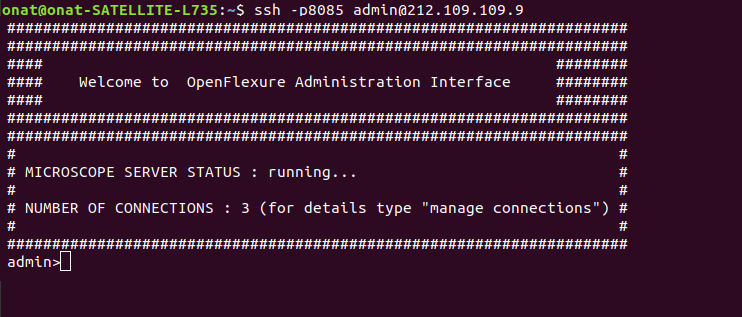
\includegraphics[scale=0.5]{Figures/admin_interface}
			\caption{OpenFlexure Administration Command-line Interface}
			\label{fig:system_admin_management_interface}
		\end{figure}
		\item \textbf{Maintainer Command-line Interface} \\
		Similar to system administrators, maintainers use a separate maintainer command-line interface to do their tasks, due to the similar reasons. Since the permissions of the maintainers are limited to viewing released updates, updating the system and retrieving the system logs, commands available to maintainers are also limited. Maintainers can list saved error logs, system details such as the current software version and the information about the latest software updates. Furthermore, maintainers are also able to update the system software using the command provided by this interface. Maintainer command-line interface is provided by a bash script placed inside the local microscope server and starts to run when a maintainer connects to the microscope using SSH.
	\end{itemize}
	\textbf{Design Rationale:} 
	\begin{enumerate}
		\item The reason to use a command-line interface rather than GUI is related to speed. Maintainers should be able to apply their actions immediately. Since the command-line interface is a more quick way to apply actions, it is preferred over GUI.
	\end{enumerate}
	\paragraph{System/Service Interfaces}
	\paragraph{Interface between Web API and Gallery}
	The interface provided by the Gallery is used by the Web API when a user sends a request to the Web API to display/edit/manage the saved media materials.
	\subparagraph{Design Rationale:}
	\begin{itemize}
		\item User sends a request to the Web API to view/edit the stored media.
		\item To allow the Web API to use the media facilities that user wants to use, Gallery provides this interface and based on the request sent to the Web API, corresponding operation of the Gallery is activated.
		\item This interface is related to the Open Gallery and Modify Media functions defined in the use-case diagram.
	\end{itemize}
	\paragraph{Interface between Web API and Position Controller}
	The interface provided by the Position Controller is used by the Web API when a user sends a request to the Web API to move the position of the stage.
	\subparagraph{Design Rationale:}
	\begin{itemize}
		\item User sends a request to the Web API to navigate the positions of the microscope stage.
		\item To allow the Web API to change the position of the stage to the desired position, Position Controller provides this interface and changes the positions of the stage using the provided coordinates.
		\item This interface is related to the Navigate Stage function defined in the use-case diagram.
	\end{itemize}
	\paragraph{Interface provided Web API and Display Controller}
	The interface provided by the Display Controller is used by the Web API when a user sends a request to display the livestream, capture the current view, record to the livestream or scan an area.
	\subparagraph{Design Rationale:}
	\begin{itemize}
		\item User sends a request to the Web API to use facilities provided by the Display Controller such as viewing livestream, capturing images, recording videos etc.
		\item To allow the Web API to use the mentioned facilities that user wants to use, Display Controller provides this interface and based on the request sent to the Web API, corresponding operation of the Display Controller is activated.
		\item This interface is related to the View Livestream, Capture Image, Record Video and Scan functions defined in the use-case diagram.
	\end{itemize}

\subsubsection{Sequence Diagrams}
\begin{figure}[H]
	\centering
	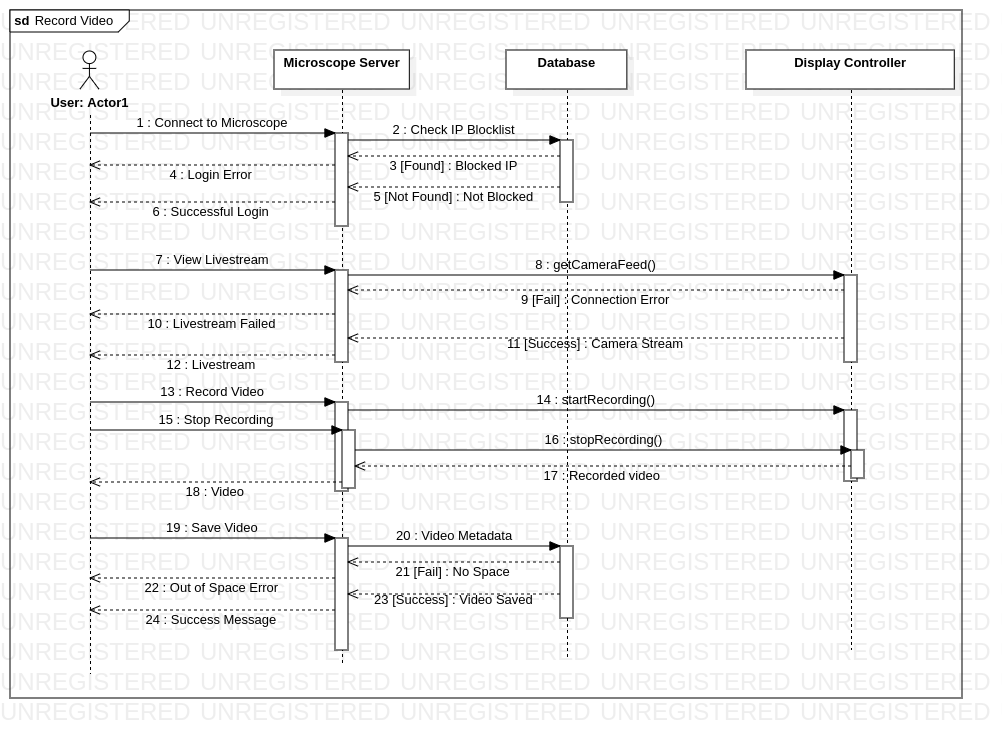
\includegraphics[scale=0.4]{Uml_Images/record_video_seq_diagram}
	\caption{Sequence Diagram of Record Video Function}
	\label{fig:record_video_seq_diagram}
\end{figure}
\begin{figure}[H]
	\centering
	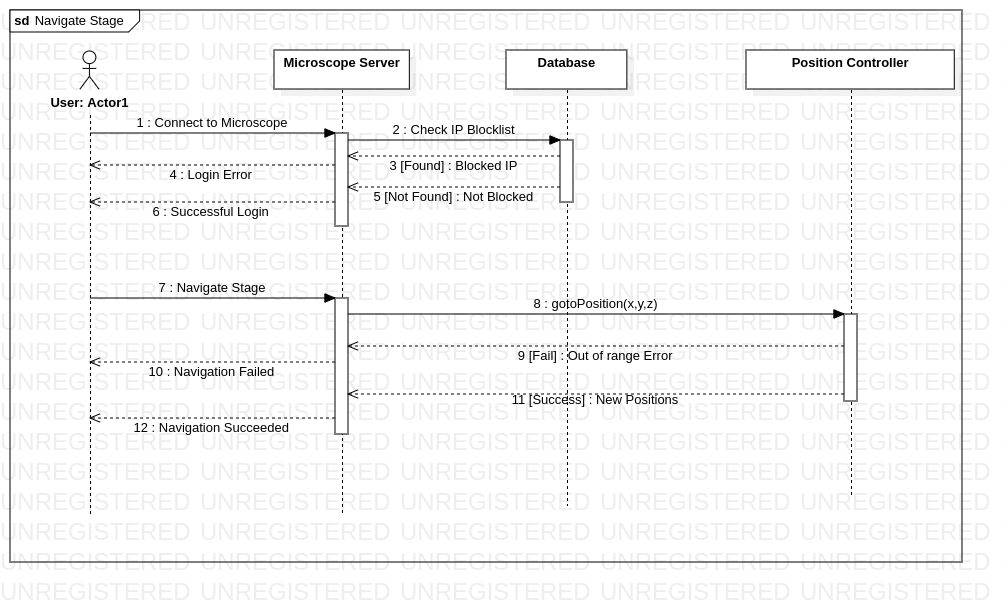
\includegraphics[scale=0.4]{Uml_Images/navigate_stage_seq_diagram}
	\caption{Sequence Diagram of Navigate Stage Function}
	\label{fig:navigate_stage_seq_diagram}
\end{figure}
\begin{figure}[H]
	\centering
	
\includegraphics[scale=0.4]{Uml_Images/block_user_seq_diagram}
	\caption{Sequence Diagram of Block User Function}
	\label{fig:block_user_seq_diagram}
\end{figure}
\begin{figure}[H]
	\centering
	
\includegraphics[scale=0.4]{Uml_Images/login_error_seq_diagram}
	\caption{Sequence Diagram of Login Error Handling}
	\label{fig:login_error_handling_seq_diagram}
\end{figure}
\begin{figure}[H]
	\centering
	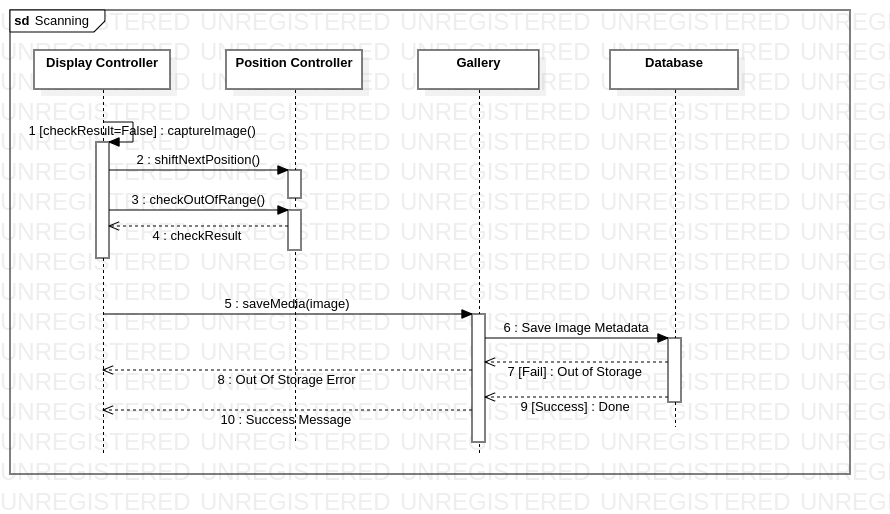
\includegraphics[scale=0.4]{Uml_Images/scanning_seq_diagram}
	\caption{Sequence Diagram of Scanning}
	\label{fig:scanning_seq_diagram}
\end{figure}
\subsubsection{Design Rationale}
Design rationales are specified where each interface is defined above.
	
	
	
	
	
\end{document}